\documentclass[10pt,letterpaper]{article}
\usepackage[top=0.85in,left=2.75in,footskip=0.75in]{geometry}
\usepackage{amsmath,amssymb}
\usepackage{changepage}
\usepackage{textcomp,marvosym}
\usepackage{cite}
\usepackage{nameref,hyperref}
\usepackage[right]{lineno}
\usepackage[nopatch=eqnum]{microtype}
\DisableLigatures[f]{encoding = *, family = * }
\usepackage[table]{xcolor}
\usepackage{array}
\usepackage{booktabs}
\newcolumntype{+}{!{\vrule width 2pt}}
\newlength\savedwidth
\newcommand\thickcline[1]{%
  \noalign{\global\savedwidth\arrayrulewidth\global\arrayrulewidth 2pt}%
  \cline{#1}%
  \noalign{\vskip\arrayrulewidth}%
  \noalign{\global\arrayrulewidth\savedwidth}%
}
\newcommand\thickhline{\noalign{\global\savedwidth\arrayrulewidth\global\arrayrulewidth 2pt}%
\hline
\noalign{\global\arrayrulewidth\savedwidth}}
\raggedright
\setlength{\parindent}{0.5cm}
\textwidth 5.25in
\textheight 8.75in
\usepackage[aboveskip=1pt,labelfont=bf,labelsep=period,justification=raggedright,singlelinecheck=off]{caption}
\renewcommand{\figurename}{Fig}
\bibliographystyle{plos2025}
\makeatletter
\renewcommand{\@biblabel}[1]{\quad#1.}
\makeatother
\usepackage{lastpage,fancyhdr,graphicx}
\usepackage{epstopdf}
\pagestyle{fancy}
\fancyhf{}
\rfoot{\thepage/\pageref{LastPage}}
\renewcommand{\headrulewidth}{0pt}
\renewcommand{\footrule}{\hrule height 2pt \vspace{2mm}}
\fancyheadoffset[L]{2.25in}
\fancyfootoffset[L]{2.25in}
\lfoot{}

\begin{document}
\vspace*{0.2in}

\begin{flushleft}
{\Large
\textbf{A computational model of the interactions between formate and insulin metabolism}
}
\newline
\\
Alexei Vazquez\textsuperscript{1*}
\\
\bigskip
\textbf{1} Nodes \& Links Ltd, Salisbury House, Station Road, Cambridge, CB1 2LA, United Kingdom
\\
\bigskip
* alexei.vazquez@gmail.com
\end{flushleft}

\section*{Abstract}
Formate, the circulating carrier of one-carbon units, supplies two carbons of
every purine ring, and cellular purine nucleotides are sensed by mTORC1 --- the
regulator of the anabolic translation the pancreatic $\beta$-cell uses to make
insulin. These links suggest an untested chain, formate $\rightarrow$ purine
nucleotides $\rightarrow$ mTORC1 $\rightarrow$ insulin synthesis, connecting
one-carbon nutrition to insulin production and diabetes risk. We formalise this
chain as a computational kinetic model calibrated to independent islet data; the
model itself --- a quantitative substrate for reasoning about formate and insulin
--- is the central contribution. Systemically, raising formate increases the
purine pool, mTOR activity and insulin synthesis, while loss of mitochondrial
formate production cuts insulin synthesis by roughly half with a parallel fall in
uric acid. Embedded in a whole-body glucose--insulin loop, this central action
raises plasma insulin, distinguishing it from a peripheral effect on glucose
uptake. An adipose compartment shows that obesity and an insulin-secretion defect
drive blood formate in opposite directions --- reconciling human cohorts that
disagree in sign --- while food formate content does not predict diabetes risk,
because the $\beta$-cell is already formate-replete. A gut-microbiome compartment
that returns urate carbon as formate closes a delayed positive-feedback urate
cycle. The retina is distinct: it makes its own insulin behind the blood-retinal
barrier, so retinal insulin tracks blood one-carbon rather than plasma insulin.
Self-regulation makes the eye a homeostat; because excess retinal insulin is
pathological, retinal health is an inverted-U in formate, and methanol optic
toxicity emerges as an acute one-carbon overload. The model turns these maps into
testable interventions: formate supplementation benefits only the
formate-deficient diabetic, and in the eye, inhibiting local formate synthesis
versus insulin synthesis is a paired, mechanism-discriminating prediction.

\section*{Author summary}
Insulin is made by specialised pancreatic cells, and too little of it causes
diabetes. I asked whether a small, common nutrient --- formate, the body's
carrier of one-carbon chemical groups --- helps set how much insulin these cells
can build. Formate supplies part of every purine, a building block of DNA and
energy molecules, and cells read their purine levels to switch on the growth
machinery (mTOR) that manufactures insulin. I built a computer model of this
chain, tuned to published measurements from insulin-producing cells, and used it
to explore what happens as formate rises and falls. The model reproduces puzzling
human data --- why blood formate can look high in some people with diabetes and
low in others --- and predicts who might benefit from formate supplements and who
would not. It also speaks to the eye, which makes its own insulin: too little or
too much formate harms the retina, and the model recasts methanol blindness as an
insulin-excess overload rather than direct poisoning of the cell's respiratory
chain. Most usefully, it proposes specific, testable experiments to confirm or
refute each prediction.

\clearpage
\newgeometry{top=0.85in,left=1in,right=1in,footskip=0.75in}
\linenumbers

\section*{Introduction}
Insulin is the body's principal anabolic hormone, and
the pancreatic $\beta$-cell that produces it is a specialised secretory factory
that couples glucose sensing both to the release of stored insulin and to the
synthesis of new hormone~\cite{rorsman2018}. Proinsulin biosynthesis is
among the most demanding acute anabolic tasks in mammalian physiology: a rise in
glucose increases total $\beta$-cell protein synthesis roughly twofold but
proinsulin synthesis ten- to twentyfold, almost entirely through translational
control~\cite{itoh1980}. Such rapid, large-scale anabolic translation is
the domain of mTOR complex~1, the master regulator that gates protein synthesis to
nutrient and energy supply~\cite{saxton2017}; accordingly, mTORC1
signalling sustains $\beta$-cell mass, insulin content and glucose-stimulated
secretion.

When insulin supply fails to meet demand, type~2
diabetes results. Obesity is the dominant driver: an expanded adipose mass
releases fatty acids, cytokines and hormones that impose systemic insulin
resistance and so raise the secretory demand on the $\beta$-cell~\cite{kahn2006}. Diabetes nevertheless emerges only when the $\beta$-cell can
no longer compensate --- $\beta$-cell dysfunction is the pivotal lesion --- within
a disease that is ultimately multi-organ, spanning islet, liver, muscle, fat, gut
and brain~\cite{defronzo2009,roden2019}. Because insulin
\emph{production} sits at the heart of this failure, any nutritional input that
modulates the $\beta$-cell's anabolic capacity is of potential relevance to
diabetes risk.

One candidate input is formate, the
circulating carrier of one-carbon units. Folate-mediated one-carbon metabolism
supplies the carbons for nucleotide, amino-acid and methylation reactions and is
highly compartmentalised: mitochondrial serine catabolism
(SHMT2--MTHFD2--MTHFD1L) oxidises serine-derived one-carbon units to formate,
which is exported to the cytosol and to the blood, and is complemented by dietary
and gut-microbial sources~\cite{ducker2017,pietzke2020}. Two carbons of every purine ring derive from formate, so formate
availability constrains de novo purine synthesis~\cite{oizel2020}. In
healthy adults, serum formate averages ${\sim}26$~$\mu$M (range $9$--$97$~$\mu$M)
and is set by its metabolic precursors (serine, methionine, choline) and by folate
status rather than by smoking or alcohol~\cite{brosnan2018}, and
circulating formate has been reported to stratify with cancer and diabetes
\cite{pietzke2019}.

These strands converge on a testable chain. Cellular
purine nucleotide levels are directly sensed by mTORC1~\cite{hoxhaj2017}, the very complex that drives insulin translation. If formate feeds the
purine pool and purines raise mTORC1 activity, then formate could act as a
nutritional modulator of insulin biosynthesis:
\textbf{formate $\rightarrow$ purine nucleotides $\rightarrow$ mTORC1 $\rightarrow$
insulin peptide synthesis}. We proposed this chain informally~\cite{spiceoflife}; it has not been tested directly. Here we build a computational
model of it --- the central contribution of this work --- and use it to
investigate, in turn, systemic insulin metabolism across formate states, retinal
insulin metabolism across formate states, and the therapeutic implications that
follow.

% ---------------------------------------------------------------------------
\section*{Results}

\subsection*{A computational model of the formate\,--\,insulin chain}
The central contribution is the model itself: a kinetic formalisation of the
proposed formate $\rightarrow$ purine $\rightarrow$ mTOR $\rightarrow$ insulin chain,
calibrated to independent islet data, that turns a verbal hypothesis into
quantitative predictions we interrogate in the parts that follow.

\subsubsection*{A kinetic $\beta$-cell model coupling formate, purines, mTOR and
insulin}
The model (\texttt{BetaCellModel}) is a system of ordinary differential
equations for 14 species in a single $\beta$-cell, with glucose as the external
input and blood formate and mitochondrial formate production as levers. Five
modules are coupled:
\begin{enumerate}\itemsep2pt
  \item \textbf{Energy metabolism.} Glucose is committed by a glucokinase-like
  sensor (Hill, half\-satu\-ra\-tion 8~mM) feeding glycolytic and oxidative ATP
  production; ATP, ADP and AMP are linked by adenylate kinase. The ATP/\allowbreak ADP ratio
  is both the anabolic fuel and, through a Hill trigger, the K-ATP/\allowbreak Ca$^{2+}$
  secretion signal.
  \item \textbf{Purine synthesis.} The formate $\rightarrow$ 10-CHO-THF
  $\rightarrow$ PRPP $\rightarrow$ PPAT $\rightarrow$ GART $\rightarrow$ ATIC
  block of the Formate-NUDT5 model, including the optional AMP/PRPP-gated
  PPAT--NUDT5 metabolite glue, terminating in IMP.
  \item \textbf{Purine degradation.} IMP, AMP and guanine nucleotides converge
  on hypoxanthine/\allowbreak xanthine and are oxidised to urate.
  \item \textbf{Uric acid secretion.} Urate is exported from the cell.
  \item \textbf{Insulin synthesis.} mTORC1 activity is a Hill function of the
  purine nucleotide pool (weighted to the guanine-nucleotide,
  de-novo-controlled pool) gated by the adenylate energy charge; it drives
  translation of pro-insulin, which matures and is secreted under the glucose
  trigger.
\end{enumerate}
Every species has an explicit rate law (mass-action / Michaelis--Menten / Hill).
The model is integrated in time to simulate transients and solved at steady
state for dose-response analysis.

\subsubsection*{Calibration to independent islet datasets}
Four modules were anchored to independent measurements, in dependency order.
(1)~\emph{Energy}: the two energy parameters were fitted so the $\beta$-cell
ATP/ADP ratio rises from \textbf{2.4 to 11.6} across 1$\rightarrow$10~mM glucose
\cite{detimary1998}, with the guanine-nucleotide pool rising in
parallel~\cite{detimary1996} and physiological ATP (0.6$\rightarrow$2.3~mM).
(2)~\emph{IMP branch}: the adenylosuccinate-synthase/lyase rates were fitted so a
low $\rightarrow$ high glucose step drops IMP (\textbf{$\times$0.25}) and raises
adenylosuccinate/S-AMP (\textbf{$\times$3.4}), reproducing Gooding et al.~\cite{gooding2015}; this required an explicit, saturable S-AMP pool. (3)~\emph{mTOR
$\rightarrow$ content}: the mTOR-independent fraction of insulin synthesis was
fitted so complete mTORC1 loss (Raptor-KO, mTOR activity $\rightarrow$0) lowers
insulin content to \textbf{50\%} of wild type~\cite{ni2017}.
(4)~\emph{GSIS}: the glucose half-saturation and basal drive of the insulin gene
were fitted to the concentration-dependent (second-phase) perifusion response
--- half-maximal secretion near 8~mM (human islets 7.9~mM) and a stimulation
index ${\sim}5$--$6$~\cite{nunemaker2006} --- giving
\textbf{EC$_{50}=8.0$~mM, stimulation index $=5.5$} (Fig~\ref{fig:cal}). The
transient first phase (peak ${\sim}1$~min) is below the model's time resolution
and was not fitted. Anchoring the granule pool to the measured $\beta$-cell
insulin content (${\sim}20$~pg/cell) puts secretion in per-cell units without
changing any calibrated ratio.

\begin{figure}[t]
  \centering
  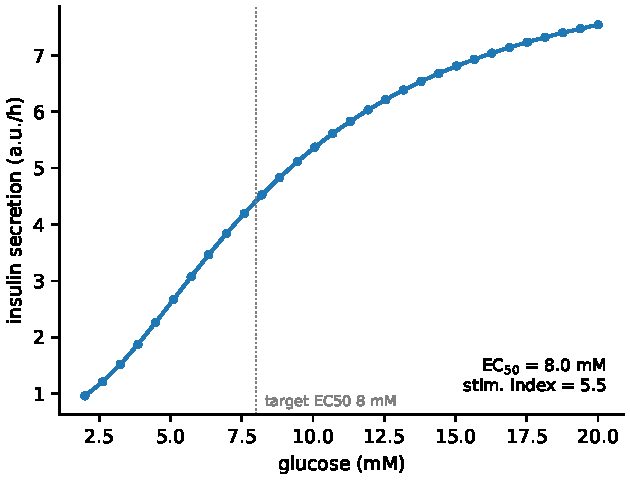
\includegraphics[width=0.52\linewidth]{fig1_calibration.pdf}
  \caption{\textbf{Calibration to GSIS.} Steady-state insulin secretion versus
  glucose after fitting to islet-perifusion benchmarks; the fitted half-maximal
  glucose (EC$_{50}$) and stimulation index are shown.}
  \label{fig:cal}
\end{figure}

\subsection*{Systemic insulin metabolism across formate states}
We first ask how systemic insulin and glucose respond as formate is varied ---
through dietary supply, mitochondrial production, and the disease states that move
blood formate --- from the isolated $\beta$-cell out to the whole body.

\subsubsection*{Formate stimulates insulin synthesis}
At stimulatory glucose (11~mM) on a formate-limited background, raising blood
formate increased the purine nucleotide pool, mTOR activity
($0.08\rightarrow0.37$) and the insulin-synthesis rate by \textbf{${\sim}66\,\%$},
saturating thereafter (Fig~\ref{fig:scan}). Uric acid secretion rose in
parallel, from 0.035 to 0.104~mM/h. The response is steep across the
physiological blood-formate range ($\le 0.3$~mM), supporting the hypothesis that
formate availability sets an anabolic ceiling on insulin production.

\begin{figure}[t]
  \centering
  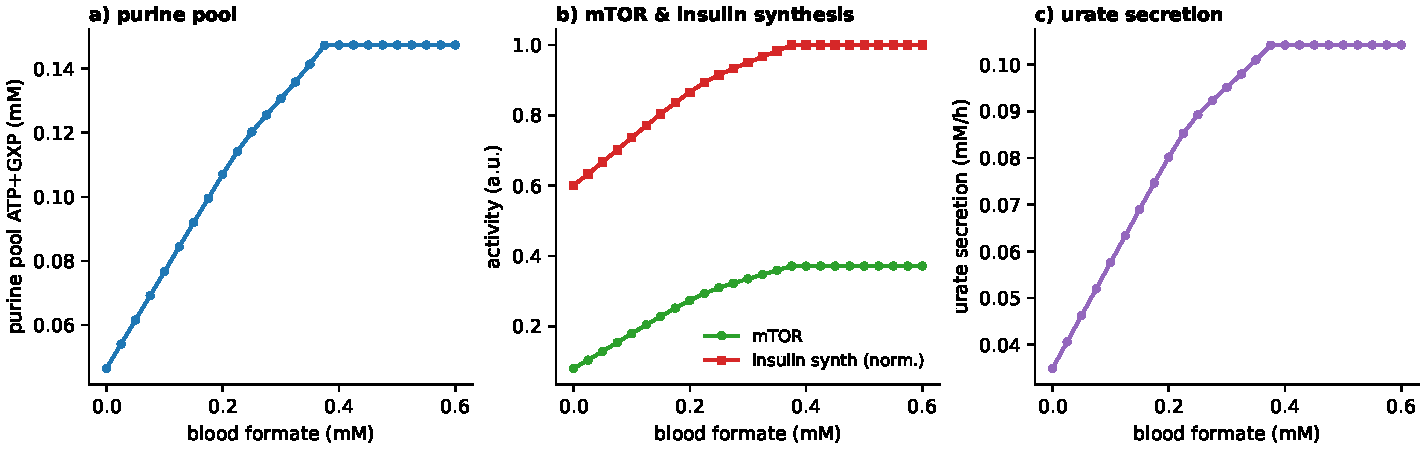
\includegraphics[width=\linewidth]{fig2_formate_scan.pdf}
  \caption{\textbf{Formate stimulates insulin synthesis.} Dietary-formate
  dose-response at 11~mM glucose on a low-endogenous-formate background. (a) purine pool; (b) mTOR activity and normalised insulin synthesis; (c) urate secretion.}
  \label{fig:scan}
\end{figure}

\subsubsection*{Mitochondrial formate deficiency impairs insulin (formate theory of
diabetes)}
We simulated formate deficiency by suppressing the endogenous mitochondrial
formate source (the MTHFD1L pathway). Lowering mitochondrial formate production
from normal to zero, at fixed 8~mM glucose, reduced intracellular formate,
collapsed mTOR activity ($0.35\rightarrow0.03$) and cut insulin synthesis by
\textbf{${\sim}45\,\%$} (Fig~\ref{fig:def}) --- the fall bounded by the
mTOR-independent synthesis floor calibrated to Ni \textit{et al}. Urate
secretion fell in parallel ($0.10\rightarrow0.02$~mM/h). The model thus predicts that a defect in
endogenous formate production --- genetic (MTHFD1L variants), mitochondrial, or
environmental (antibiotic depletion of formate-producing microbiota) ---
produces a coupled low-insulin, low-urate state, consistent with the reduced
circulating formate reported in diabetes and its seesaw with glucose
\cite{pietzke2019}. Providing dietary formate rescued insulin
synthesis on the deficient background (Fig~\ref{fig:scan}), the in-silico analog
of sodium-formate supplementation.

In a glucose-tolerance transient, a formate-replete cell entered the glucose
bolus with higher basal mTOR and a fuller granule pool and mounted a roughly
two-fold larger integrated insulin response than a formate-deficient cell
(Fig~\ref{fig:gtt}), linking chronic formate status to acute glucose tolerance.

\begin{figure}[t]
  \centering
  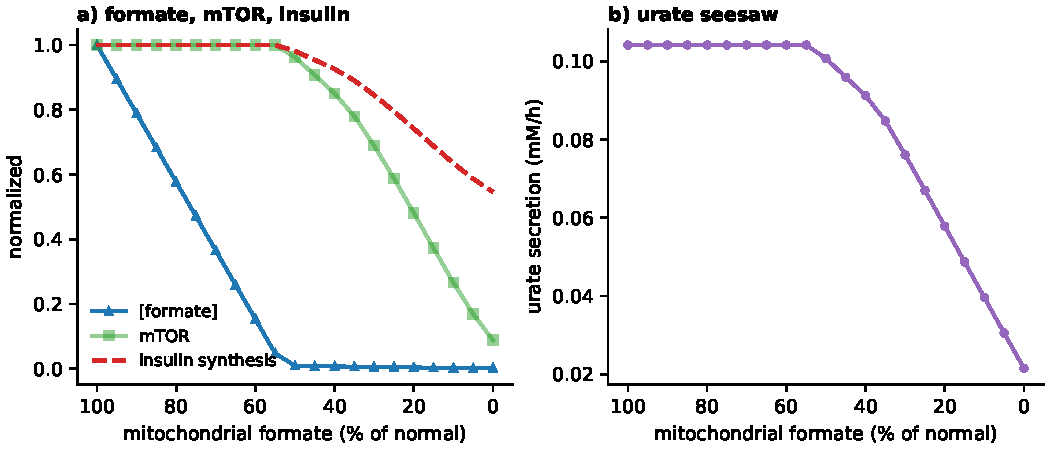
\includegraphics[width=\linewidth]{fig3_deficiency.pdf}
  \caption{\textbf{Mitochondrial-formate deficiency impairs insulin.} Suppressing
  the endogenous (MTHFD1L) formate source at 8~mM glucose. (a) intracellular formate, mTOR and insulin synthesis (normalised); (b) urate secretion falls
  with formate (the formate--urate seesaw). $x$-axis inverted: normal on the
  left, deficient on the right.}
  \label{fig:def}
\end{figure}

\begin{figure}[t]
  \centering
  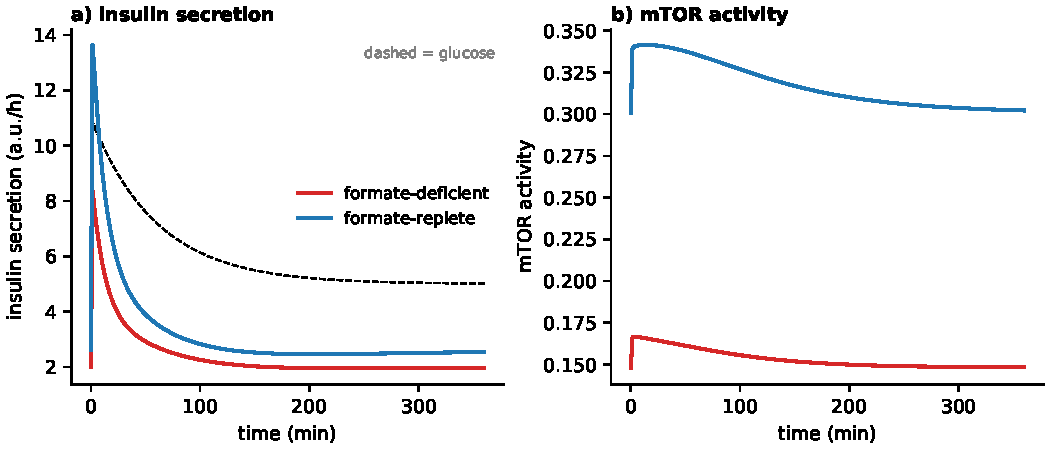
\includegraphics[width=\linewidth]{fig4_gtt.pdf}
  \caption{\textbf{Formate priming and glucose tolerance.} Glucose-tolerance
  transient (dashed: glucose bolus) for a formate-replete versus a
  formate-deficient cell, each pre-equilibrated to its basal steady state. (a) insulin secretion; (b) mTOR activity.}
  \label{fig:gtt}
\end{figure}

\subsubsection*{Sensitivity analysis isolates the controlling parameters}
Varying each assumed parameter two-fold (\texttt{data/sensitivity.csv}), we
tracked two outputs: the GSIS stimulation index (SI) and the formate sensitivity
of insulin synthesis (FS, the ratio of insulin synthesis at replete vs deficient
formate). Both outputs were insensitive (relative change $<1\,\%$) to every
insulin-secretion kinetic constant (maturation, secretion rate, secretion
trigger, ATP cost). SI was controlled by the energy/mTOR parameters (basal fuel
floor, purine-sensing Hill coefficient and half-saturation), and FS was
controlled specifically by the purine-synthesis and mTOR-sensing parameters
(purine turnover scale, mitochondrial formate capacity, the IMP-branch and
AMP-degradation rates, and the purine-sensing Hill coefficient). The
formate $\rightarrow$ insulin prediction therefore rests on the identifiable
purine/mTOR module and not on the loosely-constrained secretion kinetics.

\subsubsection*{A whole-body loop discriminates central from peripheral formate
action}
The central prediction --- formate improves glucose tolerance by raising
$\beta$-cell insulin synthesis --- must be separated from the alternative that
formate (via methylamine/AOC3) raises \emph{insulin-independent} peripheral
glucose uptake~\cite{carpene2019}. We embedded the $\beta$-cell as
the insulin source of a Bergman-type minimal model of blood glucose, plasma
insulin and remote insulin action (\texttt{WholeBody}). In this framework
the peripheral mechanism is precisely an increase in glucose effectiveness
($S_g$), the insulin-independent disposal term. We simulated a glucose-tolerance
test under formate acting centrally (through the mechanistic $\beta$-cell),
peripherally (raising $S_g$), or both, tuning the peripheral effect so that it
lowered the glucose excursion by the same amount as the central one
(Fig~\ref{fig:wb}).

Both mechanisms lowered the glucose area-under-the-curve (central $-21\,\%$,
peripheral $-14\,\%$), but they were cleanly separated by plasma insulin: the
central mechanism \emph{raised} the insulin AUC by $20\,\%$, whereas the
peripheral mechanism left it essentially unchanged ($-2\,\%$; slightly lower,
because the reduced glucose excursion drives less secretion). The model therefore
yields a
concrete discriminating experiment: \textbf{during a formate-supplemented
glucose-tolerance test, measure plasma insulin} --- a rise indicates the central
($\beta$-cell synthesis) mechanism of \textit{The Spice of Life}~\cite{spiceoflife}, whereas
unchanged or lower insulin at improved glucose tolerance indicates the peripheral
mechanism of Carp\'ene \textit{et al}. The two are not mutually exclusive; the
``both'' scenario shows their glucose effects add while the insulin signature
follows the central arm.

\begin{figure}[t]
  \centering
  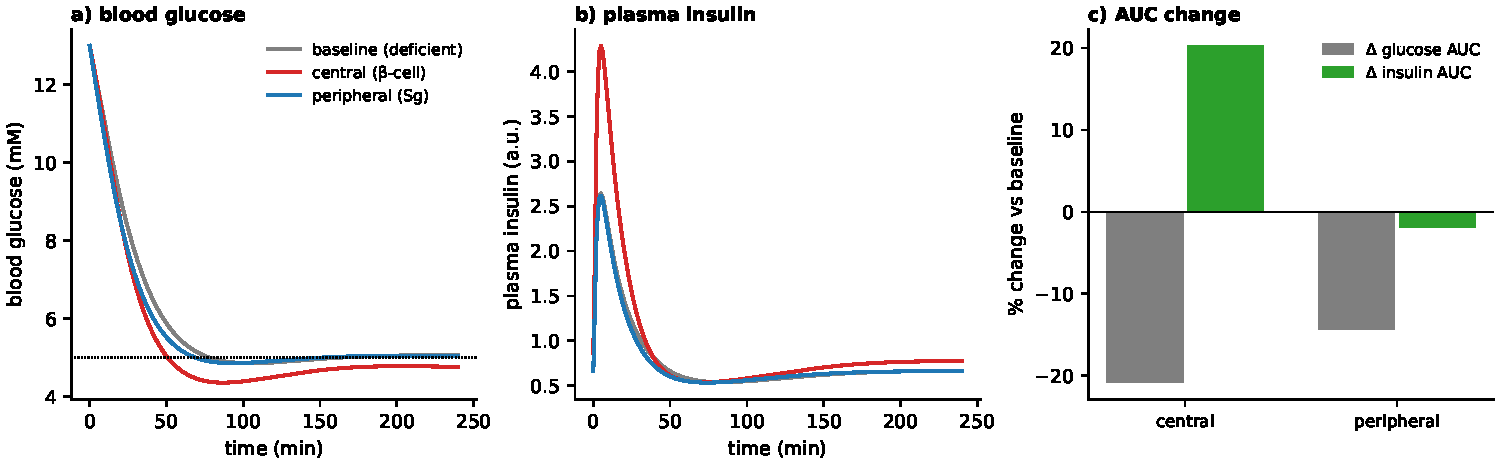
\includegraphics[width=\linewidth]{fig5_wholebody.pdf}
  \caption{\textbf{Plasma insulin discriminates the site of formate action.}
  Whole-body glucose-tolerance test with formate acting centrally
  ($\beta$-cell insulin synthesis) or peripherally (glucose effectiveness $S_g$),
  matched to the same glucose lowering. (a) blood glucose (central $\approx$ peripheral); (b) plasma insulin (separates them); (c) change in glucose and insulin AUC versus baseline --- same glucose, opposite insulin.}
  \label{fig:wb}
\end{figure}

\subsubsection*{Reconciling the formate--diabetes paradox}
A large prospective cohort (Takase et al.~\cite{takase2025}; TMM CommCohort,
$n=12{,}461$, 354 incident cases) reports circulating formic acid \emph{positively}
associated with incident type~2 diabetes (relative risk 1.45, 95\%~CI
1.11--1.91 per 1-SD), the \emph{opposite} of the low-formate reading of the
deficiency route. We asked whether the model can nonetheless reproduce this. The
model admits two distinct routes to diabetes: (A)~formate \emph{deficiency}, which
lowers insulin and predicts \emph{low} formate; and (B)~a primary insulin-\emph{
secretion} defect --- the genetically driven diabetes of the cohort --- which is
independent of formate. Because insulin is the anabolic hormone that drives de
novo purine synthesis, and purine synthesis is the principal formate \emph{sink},
route~(B) predicts that impaired insulin lets formate \emph{overflow} upward.

We tested this by promoting blood formate to a dynamic pool ---
$\dot{F}_b = \text{intake} + \text{endogenous} - U(\text{insulin},F_b) - k_{\mathrm{ren}}F_b$,
with the consumption $U$ scaling with plasma insulin --- on top of the whole-body
loop, and imposing a graded secretion defect (\texttt{FormateDiabetes}). As
secretion is impaired, blood glucose rises (4.8$\rightarrow$7.8~mM) and blood
formate rises \textbf{$\times$1.5--1.6 at every dietary serine/formate intake}
(0.8$\rightarrow$1.3, 1.6$\rightarrow$2.6 and 4.4$\rightarrow$6.4~mg/L for low,
normal and high intake; Fig~\ref{fig:diab}), yielding a positive
formate--glucose association from reduced formate \emph{utilisation} rather than
causation. This is consistent with the cohort's own internal evidence: formate
did not differ by genetic risk (11.3 vs 11.2, $P=0.77$) and was not a mediator of
the polygenic-risk $\rightarrow$ diabetes effect, i.e. it behaves as a downstream
consequence marker, exactly as route~(B) predicts. The model therefore produces
\emph{either} low formate (deficiency-route diabetes~\cite{pietzke2019}) \emph{or}
high formate (secretion-defect diabetes~\cite{takase2025}), and the two are told apart
by the accompanying insulin: overflow occurs with \emph{low} insulin and high
glucose.

\begin{figure}[t]
  \centering
  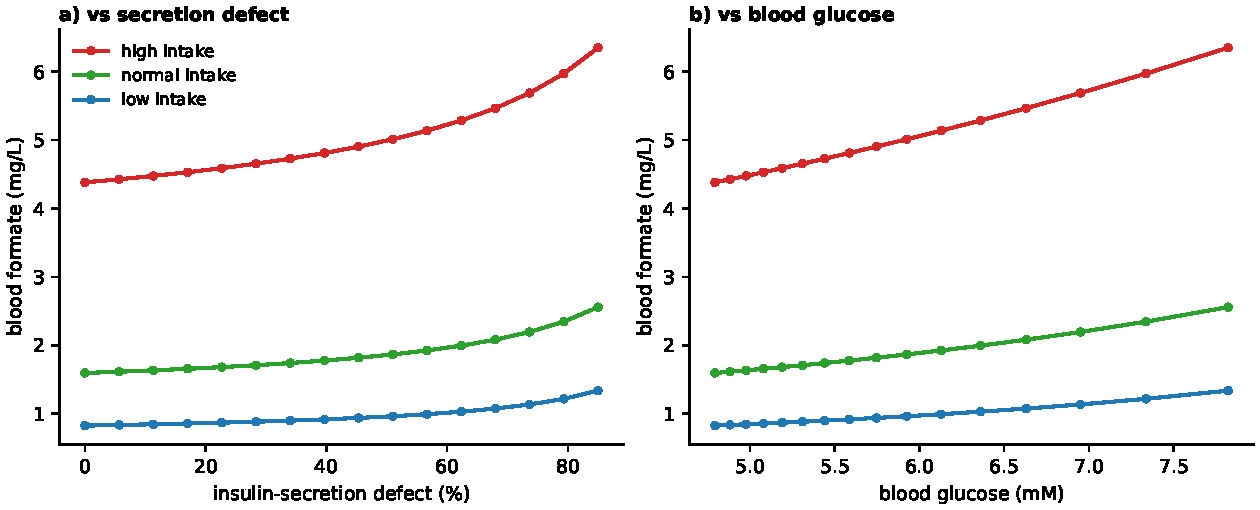
\includegraphics[width=\linewidth]{fig6_formate_diabetes.pdf}
  \caption{\textbf{A secretion defect makes blood formate overflow.} Blood formate
  versus the insulin-secretion defect (a) and versus blood glucose (b), at
  low/normal/high dietary serine--formate intake. Impaired secretion raises both
  glucose and formate at every intake, reproducing the positive formate--diabetes
  association of Takase et al.~\cite{takase2025} as reduced insulin-driven
  consumption, not causation.}
  \label{fig:diab}
\end{figure}

\subsubsection*{Obesity and diabetes move blood formate in opposite directions}
The two cohorts that bracket the human evidence disagree in sign: severe obesity
carries \emph{low} formate~\cite{pietzke2019} whereas incident diabetes in a
largely non-obese population carries \emph{high} formate~\cite{takase2025}. We asked
whether a third compartment --- adipose tissue --- resolves this. We built a
metabolic model of the adipocyte (\texttt{AdipocyteModel}) reusing the same energy
and one-carbon/purine machinery as the $\beta$-cell but with insulin-dependent
glucose uptake and lipid storage in place of insulin synthesis. Adipose plays two
formate-relevant roles: it is a one-carbon \emph{sink} (blood formate
$\rightarrow$ de novo purine) and, through xanthine oxidoreductase, a uric-acid
\emph{source} whose activity and mass both rise in obesity~\cite{tsushima2013}. Coupling the $\beta$-cell, the adipocyte and shared blood pools
(glucose, insulin, formate, urate; \texttt{CoupledModel}), we crossed
obesity (adipose mass $\times$3, XOR $\times$2, insulin resistance) with diabetes
(secretion defect).

The two axes move blood formate oppositely (Fig~\ref{fig:obes}). Obesity alone
\emph{lowers} blood formate ($-14\,\%$) --- the expanded adipose sink consumes it
--- while \emph{raising} blood uric acid ($+4\,\%$), matching Pietzke and Tsushima.
Diabetes alone \emph{raises} blood formate ($+21\,\%$) by the secretion-defect
overflow of the previous section. In the combined obese-diabetic state the two
nearly cancel ($+5\,\%$), and uric acid is highest ($+5\,\%$). The model thus
predicts that the sign of the formate--diabetes association depends on how much
obesity accompanies the diabetes: an obesity-dominated cohort sees low formate,
a secretion-defect-dominated (leaner) cohort sees high formate --- reconciling
the two datasets within one mechanism, and simultaneously reproducing the
obesity--hyperuricaemia link.

\begin{figure}[t]
  \centering
  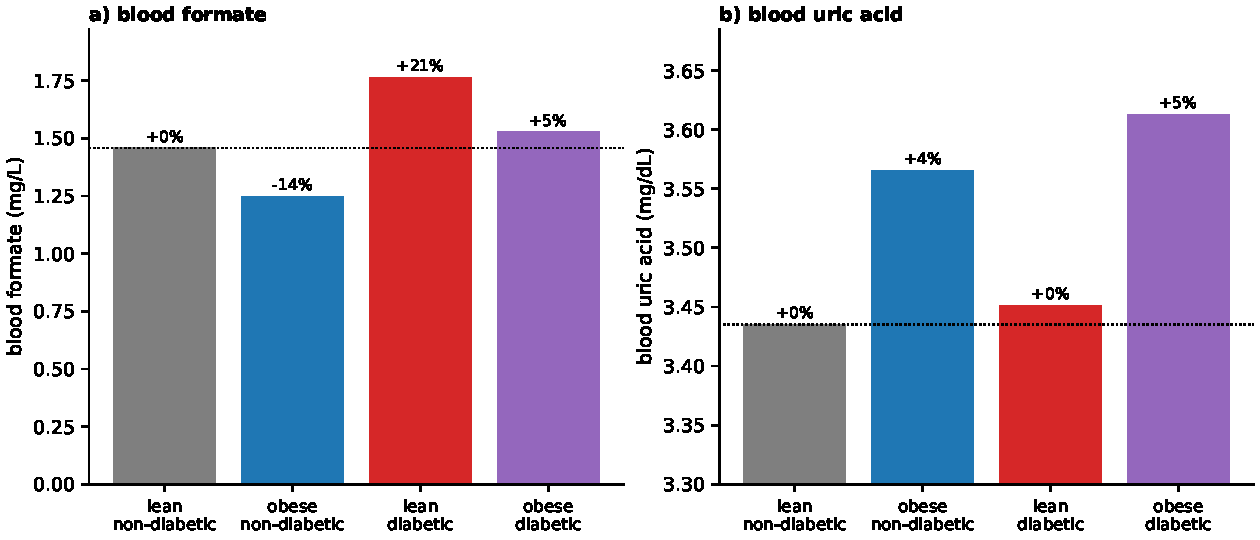
\includegraphics[width=\linewidth]{fig7_obesity_diabetes.pdf}
  \caption{\textbf{Obesity and diabetes push blood formate opposite ways.}
  Three-compartment model (pancreas + adipose + blood). (a) blood formate falls with obesity (adipose one-carbon sink) and rises with diabetes (secretion-defect overflow); the obese-diabetic state is intermediate. (b) blood uric acid
  rises with obesity via adipose XOR~\cite{tsushima2013}. Percentages are relative to
  the lean non-diabetic state.}
  \label{fig:obes}
\end{figure}

\subsubsection*{The gut microbiome closes a urate cycle: a delayed positive
feedback}
Urate is the end product of purine catabolism and is usually treated as a
metabolic dead end, cleared renally and intestinally. But the gut microbiome
degrades urate anaerobically, and this bacterial purine metabolism is now
recognised as a major contributor to host purine homeostasis~\cite{kasahara2023}. The \emph{urate cycle} hypothesis~\cite{vazquez2020urate} proposes
that this closes a loop: of the five urate carbons the microbiome returns three
--- the two glycine-derived carbons as acetate (feeding lipogenesis) and one of
the two purine formate carbons as formate itself --- so that
formate $\rightarrow$ de~novo purine $\rightarrow$ urate $\rightarrow$ (gut)
$\rightarrow$ formate becomes a cycle, with the co-produced acetate a candidate
driver of the obese metabolic signature.

We added a gut-microbiome compartment (\texttt{GutUrateCycle}): blood urate is
taken up by the gut route (diverting it from renal loss) and returned to the
circulation as formate after a processing/transit delay, modelled as a linear
chain of compartments (mean lag $\tau_{gut}$). Three features emerge
(Fig~\ref{fig:gut}). First, the return \emph{recovers urate carbon as formate}:
switching the cycle on raises blood formate (lean ${\sim}1.5\rightarrow2.3$~mg/L,
obese ${\sim}1.25\rightarrow2.0$~mg/L) while lowering circulating urate, now partly
cleared through the microbiome rather than accumulating (Fig~\ref{fig:gut}b).
Second, it is a \emph{bounded} positive feedback: because only one of the two
purine formate carbons is recycled, the loop gain is below one, so blood formate
rises smoothly and \emph{converges} as the gut recycling strengthens ---
self-reinforcing but stable, not runaway (Fig~\ref{fig:gut}c). Third, the gut
delay makes it a \emph{lagged} feedback: a purine/urate load (a purine-rich meal)
clears from the blood within a few hours but returns as a secondary blood-formate
rise ${\sim}\tau_{gut}$ (${\sim}12$~h) later (Fig~\ref{fig:gut}d) --- a signature
the closed loop predicts and against which a labelled purine bolus could be timed.

This places obesity inside the loop: the adipose xanthine-oxidoreductase induction
that raises urate in obesity (above) supplies the cycle with more substrate, while
the co-produced acetate feeds fatty-acid and cholesterol synthesis --- the
hypothesised route from urate to weight gain~\cite{vazquez2020urate} --- which nominates
the gut urate step, rather than host xanthine oxidase, as a more specific
therapeutic target. (The model captures the formate-recycling arm quantitatively;
the acetate $\rightarrow$ lipogenesis arm is represented only as a noted output, and
the delay, yield and gut-uptake rate are assumed, so the robust content is the
qualitative behaviour: carbon recovery, bounded feedback, and delayed return.)

\begin{figure}[t]
  \centering
  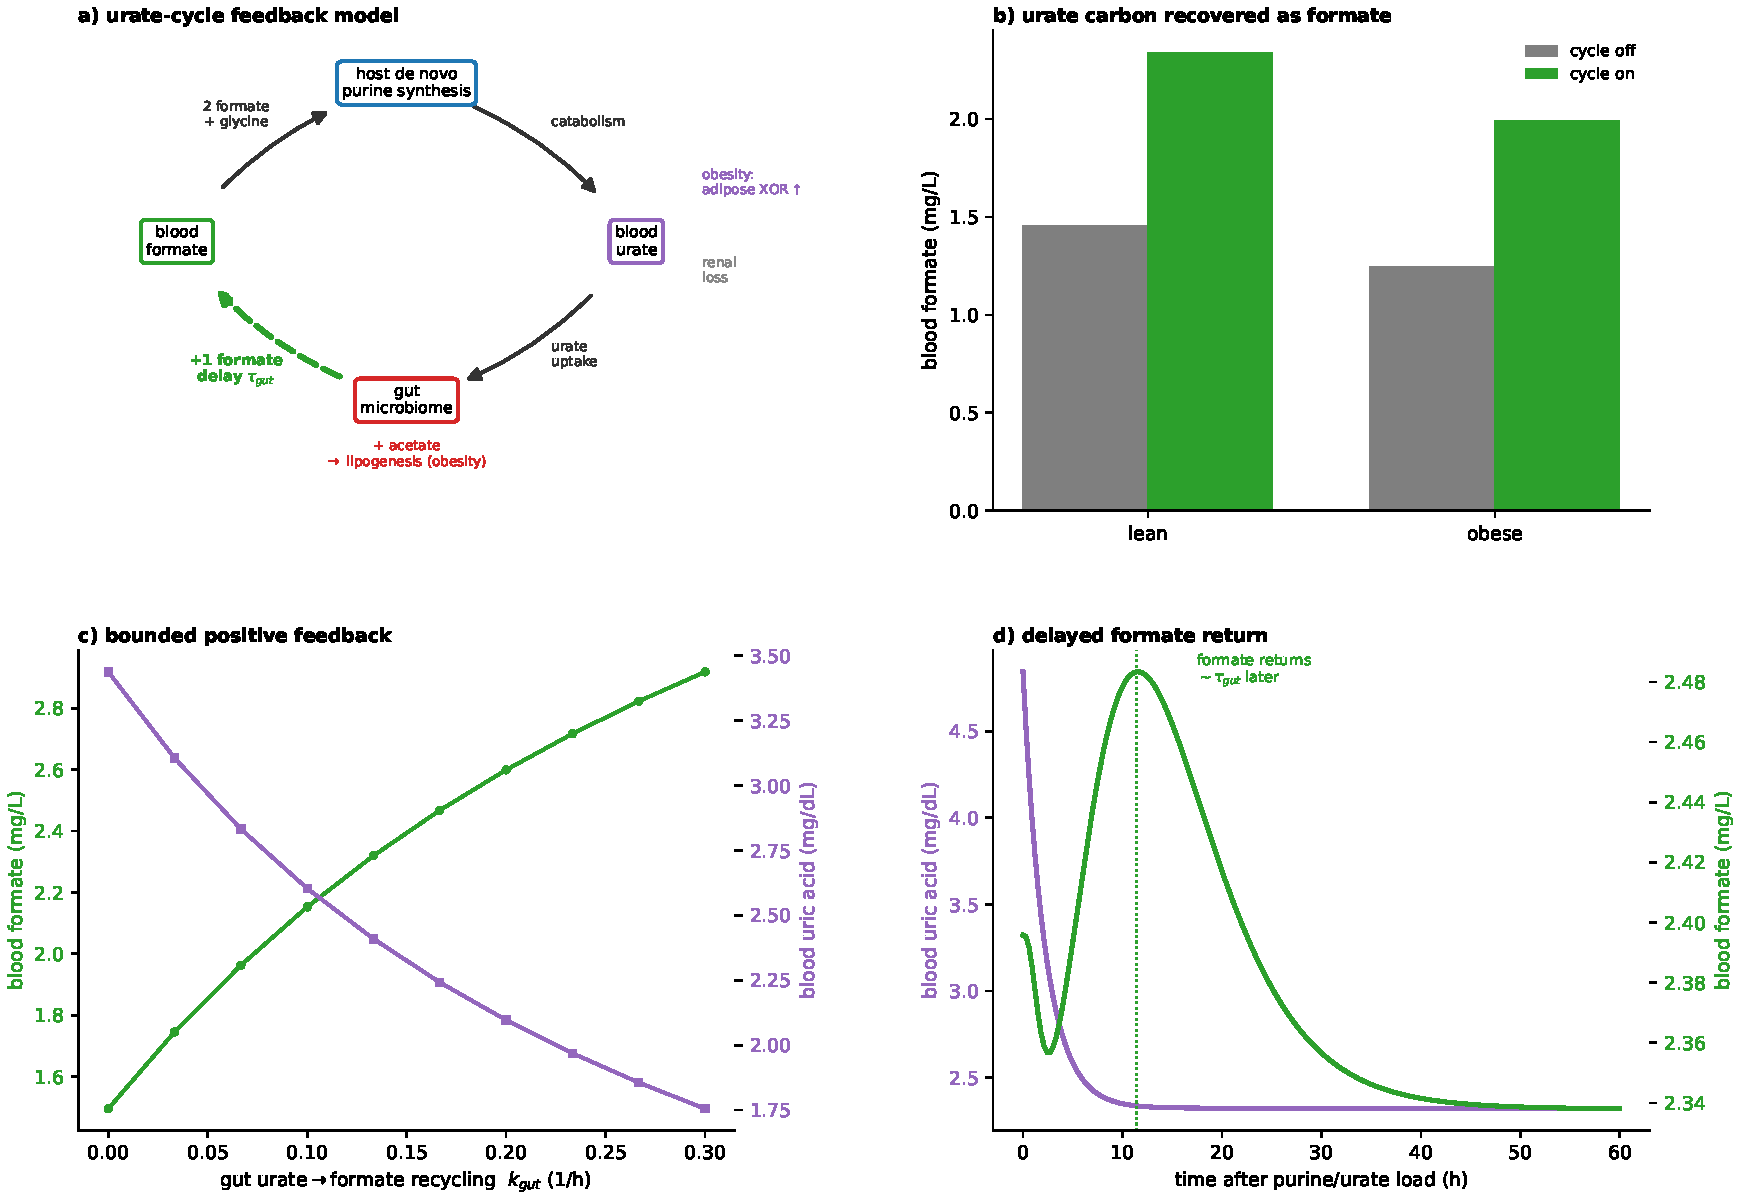
\includegraphics[width=\linewidth]{fig22_urate_cycle.pdf}
  \caption{\textbf{The gut microbiome closes a urate cycle: a delayed positive
  feedback.} A gut-microbiome compartment degrades blood urate and returns formate
  after a delay $\tau_{gut}$. (a) Schematic of the model: host purine synthesis
  consumes two formate (plus glycine) per urate; the gut microbiome returns one of
  them as formate after the delay $\tau_{gut}$ (green, closing the loop) and
  co-produces acetate ($\rightarrow$ lipogenesis). (b) Steady-state blood formate
  with the cycle off versus on, lean and obese --- urate carbon is recovered as
  formate. (c) As the gut urate $\rightarrow$ formate recycling $k_{gut}$
  strengthens, blood formate rises and blood urate falls, both converging: a
  bounded positive feedback (loop gain $<1$). (d) A purine/urate load clears from
  the blood within hours but returns as a blood-formate rise ${\sim}\tau_{gut}$
  ($\sim$12~h) later.}
  \label{fig:gut}
\end{figure}

\subsubsection*{Diet: food formate does not predict systemic glucose}
The dietary sources of formate differ enormously per serving. Whole foods
dominate~\cite{spiceoflife}: ${\sim}1000$~mg from 1~g creatine,
700~mg from 200~g meat, 70--600~mg per litre of fruit juice. Caffeine- and
aspartame-containing drinks and medications contribute far less; for these we use
the formate-generation potential tabulated by Pietzke et al.~\cite{pietzke2020} (Table~2) --- the formaldehyde released by demethylation of caffeine and
aspartame, taken to full conversion to formate --- which gives ${\sim}43$~mg per
diet cola, ${\sim}37$~mg per diet soda, ${\sim}31$~mg per cup of brewed coffee,
${\sim}8$~mg per regular cola, and up to ${\sim}47$~mg per caffeine pill
(Fig~\ref{fig:formate}). (The commonly cited ``$80$~mg per diet cola'' is the
aspartame \emph{mass}, not the formate it yields.) If dietary formate set glucose
control, these should rank foods by benefit. We tested this against a
meta-analysis of the glucose/diabetes literature for each item and against the
model.

The ranking fails. Pooling the best available estimates for incident type~2
diabetes per serving --- coffee RR~0.91 (0.89--0.94~\cite{ding2014}),
sugar-sweetened cola RR~1.13 and 100\% fruit juice RR~1.07 and artificially
sweetened (diet) cola RR~1.08~\cite{imamura2015}, red meat HR~1.10
per 100~g~\cite{li2024}, and creatine glycaemically neutral in
randomized trials (fasting-glucose SMD~$+0.05$, HOMA-IR SMD~$-0.38$, both
non-significant~\cite{delpino2022}) --- the correlation between a food's
formate content and its diabetes effect is essentially zero ($r=-0.03$;
Fig~\ref{fig:diet}). Coffee, near the bottom of the formate table, is the
only protective item; creatine and meat, at the top, are neutral and harmful.
Each food's glycaemic effect is carried by its dominant components --- sugar,
saturated fat, chlorogenic acids --- not its formate.

The model predicts exactly this null. Because the pancreatic $\beta$-cell is
already formate-replete, adding dietary formate raises blood formate (${\sim}3$-fold
across the range of foods; Fig~\ref{fig:formate}) but leaves plasma insulin
and fasting glucose flat --- unchanged across every food, and so not plotted;
systemic glucose control is therefore governed by
what else the food carries, not by its formate. Consistent with this, the two
foods with any glycaemic benefit act by \emph{insulin-independent} routes ---
creatine through GLUT4 translocation (with exercise), coffee through non-caffeine
components (caffeinated and decaffeinated coffee are equally protective) --- not
through $\beta$-cell insulin. The one place dietary formate does register in the
model is not systemic at all but ocular --- a prediction we take up with the
retinal model (below).

\begin{figure}[t]
  \centering
  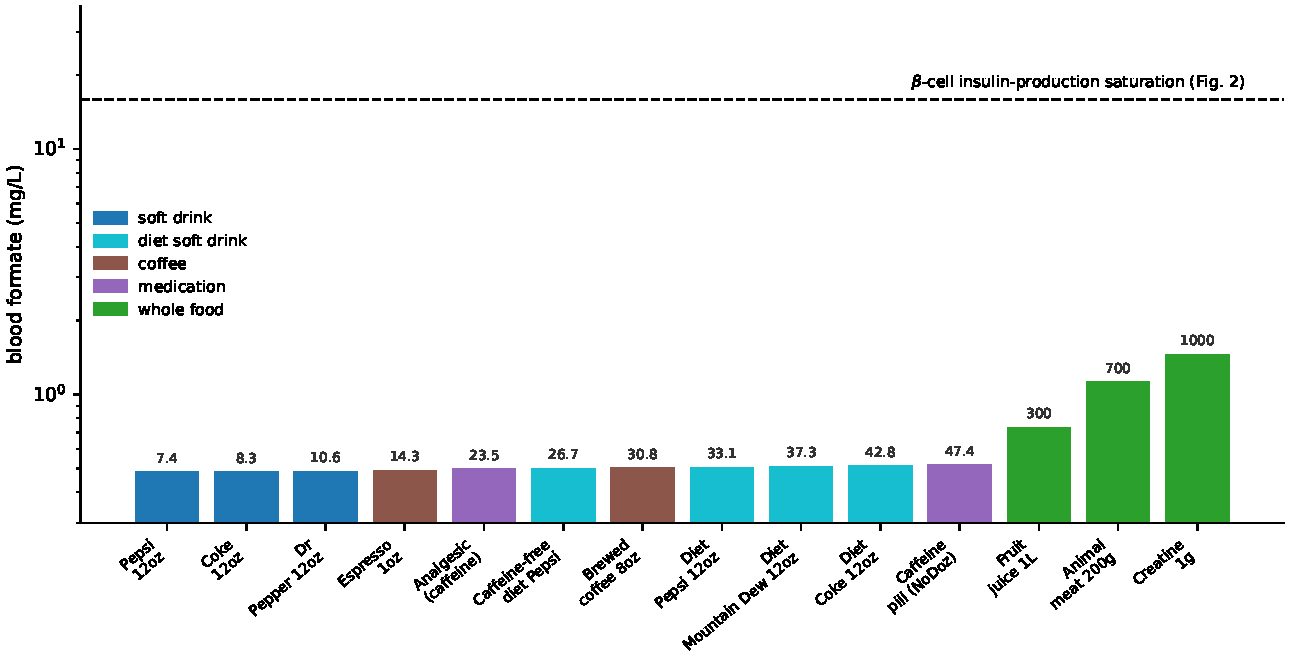
\includegraphics[width=\linewidth]{fig14_diet_formate.pdf}
  \caption{\textbf{Blood formate delivered by each food/beverage.} Model-predicted
  blood formate for the caffeine/aspartame drinks and medications of
  \cite{pietzke2020} Table~2 (coloured by category, formate per serving annotated) plus
  the whole-food sources; all the beverages and pills deliver near-baseline blood
  formate, spanning ${\sim}3$-fold only once the high-content whole foods (fruit
  juice, meat, creatine) are included. The dashed line marks the blood-formate
  level that saturates $\beta$-cell insulin production (Fig~\ref{fig:scan},
  ${\sim}0.3$~mM); every food lies more than an order of magnitude below it (note
  the log axis), so dietary formate cannot drive systemic insulin.}
  \label{fig:formate}
\end{figure}

\begin{figure}[t]
  \centering
  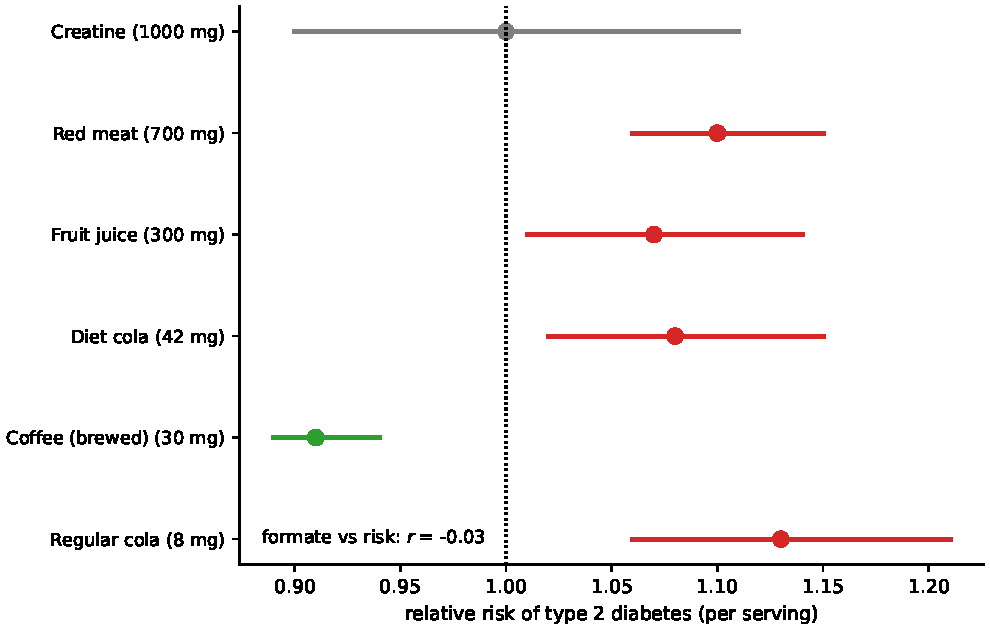
\includegraphics[width=0.68\linewidth]{fig15_diet_forest.pdf}
  \caption{\textbf{Food formate does not predict the diabetes effect.}
  Meta-analytic relative risk of type~2 diabetes per serving for the six items
  with a per-serving estimate (beverage formate contents from~\cite{pietzke2020}
  Table~2), ordered by formate content (mg per serving in parentheses); the
  formate ranking is uncorrelated with the effect ($r=-0.03$). Coffee (low
  formate) is protective while creatine and meat (high formate) are neutral and
  harmful.}
  \label{fig:diet}
\end{figure}

\subsection*{Retinal insulin metabolism across formate states}
The retina is a special case. It makes its own insulin behind the blood-retinal
barrier, so retinal insulin tracks blood one-carbon rather than plasma insulin. We
give it a dedicated compartment and follow its insulin from deficiency, through a
physiological optimum, to the toxic excess of methanol.

\subsubsection*{The eye: a self-regulating one-carbon compartment}
The retina makes its own insulin: the retinal pigment epithelium (RPE) produces
and secretes insulin locally, stimulated by photoreceptor phagocytosis, to
support cone survival and regeneration, and it does so even under systemic insulin
deficiency or resistance~\cite{etchegaray2023}. The blood-retinal
barrier keeps \emph{circulating} insulin out of the eye, so the retina cannot
borrow plasma insulin --- but small molecules, including glucose and one-carbon
units (serine/formate), do cross. We therefore added an eye compartment
(\texttt{EyeModel}): a retinal insulin-producing cell running the same
formate $\rightarrow$ purine $\rightarrow$ mTOR $\rightarrow$ insulin machinery as the
$\beta$-cell, driven by blood glucose and blood formate, with its insulin kept
strictly local and a low endogenous mitochondrial formate. Local insulin drives a
retinal maintenance/regeneration index. Supplied only from the blood, eye insulin
rises monotonically with circulating formate (Fig~\ref{fig:local}, blue).

\emph{Does the eye also make its own formate, co-regulated with the insulin it
produces?} Two lines of evidence say partly yes. First, single-cell expression
(Human Protein Atlas; Fig~\ref{fig:expr}): the insulin-producing RPE expresses
the one-carbon \emph{entry} enzymes SHMT2 and MTHFD2 at modest levels but is
\emph{depleted} for the formate-\emph{releasing} enzyme MTHFD1L, which instead
peaks in the adjacent cone photoreceptors (the eye's highest, ${\sim}46\times$ the
RPE) --- the very outer segments the RPE phagocytoses to trigger its insulin.
Second, the mechanism: mTORC1 $\rightarrow$ ATF4 is the master inducer of
SHMT2/MTHFD2~\cite{bensahra2016}, and in islets the same ATF4
program that raises insulin content co-induces this serine-linked one-carbon
pathway~\cite{pelligra2023}; phagocytosing RPE activates ATF4 as its
top upstream regulator. We could not find a dataset that directly measures these
enzymes rising with \textit{Ins2} in the RPE, so the co-induction is, for now,
strong inference rather than eye-level measurement.

We encoded it as a feed-forward: the eye cell's local formate production is
induced by its own mTOR/insulin-synthesis signal (lumping the RPE's ATF4-driven
one-carbon entry with the cone-paracrine, MTHFD1L-rich formate supply). Left
unregulated this runs away --- eye insulin is pinned at its formate-saturated
maximum (${\sim}2.62$~a.u., well above the retinal optimum of $\sim$1.98;
Fig~\ref{fig:local}, red) --- which is biologically implausible: local retinal
insulin is homeostatically controlled. Two mechanisms do so, both documented in
the RPE. Production is not constitutive but \emph{signal-gated} --- switched on by
MerTK-dependent phagocytosis of photoreceptor outer segments, a circadian pulse
amplified by starvation~\cite{etchegaray2023}. And insulin/IGF
signalling is capped by the mTORC1 $\rightarrow$ S6K1 $\rightarrow$ IRS-1
negative-feedback loop, shown directly in RPE cells~\cite{leontieva2014}; indeed the proliferative retinopathy of chronic ocular IGF-1 excess
\cite{ruberte2004,villacampa2013} reads as loss of exactly this cap. Adding the
S6K1 $\rightarrow$ IRS-1 feedback tames the feed-forward: across the physiological
range of blood formate the regulated eye holds local insulin near the retinal
optimum (${\sim}1.9$--$2.0$; Fig~\ref{fig:local}, green) --- \emph{lifted} toward
the optimum at the low circulating formate of obesity or metformin, where the
blood-dependent eye is deficient, and overridden into excess only when
\emph{external} formate climbs above the physiological range.

Because a positive feed-forward can in principle produce bistability (a switch
with hysteresis), we characterized the regulated eye before using it. Basin tests
(integrating from many initial conditions at each condition) and a
self-consistency/bifurcation analysis agree (Fig A in S1 Appendix): the
response is \emph{monostable} --- a single stable steady state at every blood
formate and glucose, with no hysteresis, and no bistability even at five-fold the
reference feed-forward gain (the S6K1 cap prevents it). The regulated eye is
therefore a smooth homeostat, not a switch; were the retina's insulin pulse
switch-like (it is circadian), that behaviour would come from the phagocytosis
signal-gate, not from this metabolic loop.

Across the clinical conditions the prediction is a clean dissociation
(Fig~\ref{fig:eye}). The regulated eye insulin sits near the retinal optimum but
is decoupled from \emph{plasma} insulin: it \emph{anti-}correlates with plasma
insulin ($r=-0.90$) and tracks blood one-carbon and local glucose ($r=+0.89$ with
blood formate). The lean healthy and obese non-diabetic states, which carry the
\emph{highest} plasma insulin, sit just \emph{below} the optimum (mild
deficiency); the lean secretion-defect diabetic --- lowest plasma insulin, but
highest blood formate and hyperglycaemic --- is pushed \emph{above} the optimum
into mild retinal-insulin excess. Retinal insulin status is thus governed by blood
one-carbon and local glucose, not by systemic insulin: states that lower blood
formate (obesity's adipose sink; metformin's SHMT2 inhibition) pull the retina
toward the deficient side even as systemic glucose improves, while serine/formate
raise it (a candidate mechanism relevant to diabetic retinopathy, and consistent
with the ocular tolerability of formate supplementation~\cite{altaweel2009}).

\begin{figure}[t]
  \centering
  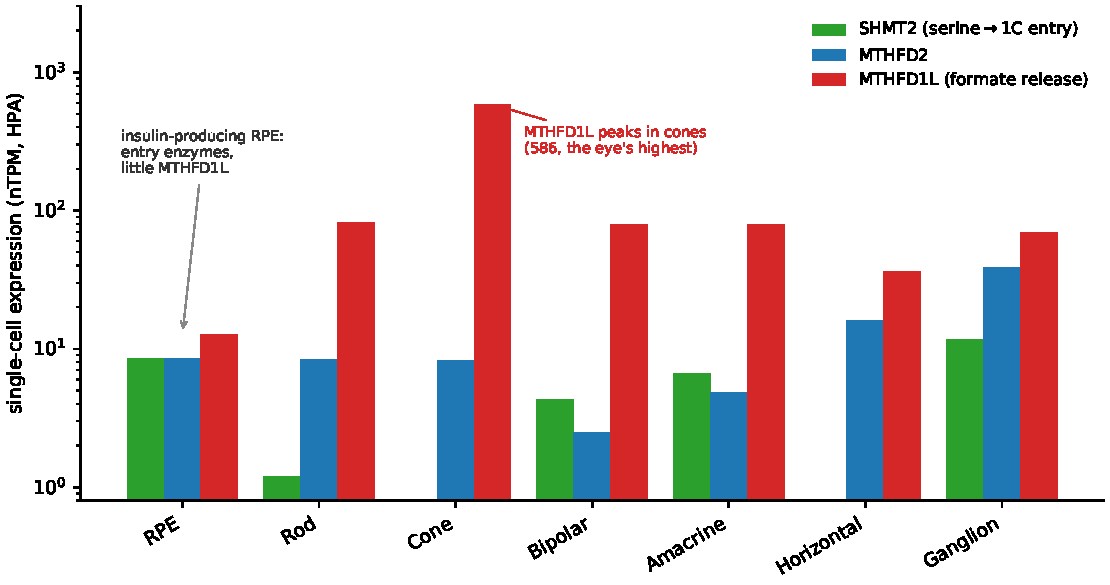
\includegraphics[width=0.82\linewidth]{fig17_eye_onecarbon.pdf}
  \caption{\textbf{One-carbon/formate enzymes across eye cell types.} Single-cell
  expression (Human Protein Atlas, log scale) of SHMT2 and MTHFD2 (one-carbon
  entry) and MTHFD1L (formate release). The insulin-producing RPE has the entry
  enzymes but little MTHFD1L; the formate-releasing enzyme peaks in cone
  photoreceptors --- the outer segments the RPE phagocytoses.}
  \label{fig:expr}
\end{figure}

\begin{figure}[t]
  \centering
  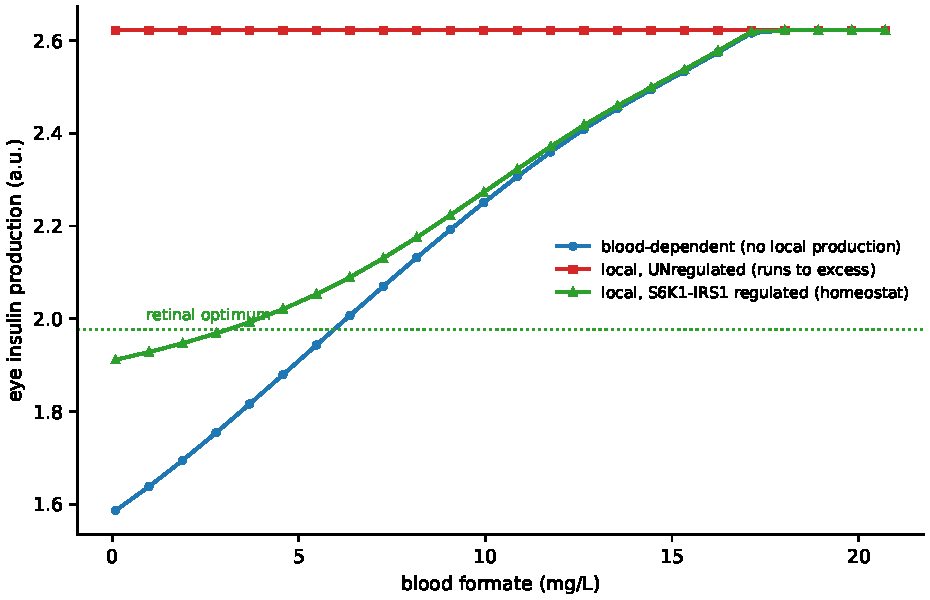
\includegraphics[width=0.62\linewidth]{fig18_eye_local.pdf}
  \caption{\textbf{Local co-induced formate: runaway versus regulated homeostat.}
  Predicted eye insulin versus blood formate at fixed glucose. Blood-dependent
  (blue) rises with circulating formate. The unregulated ATF4 feed-forward (red)
  runs away to the formate-saturated maximum, in the insulin-excess zone above the
  retinal optimum. Adding the S6K1 $\rightarrow$ IRS-1 negative feedback (green)
  makes local production homeostatic: across the physiological range eye insulin
  is held near the optimum --- lifted toward it at low blood formate, where the
  blood-dependent eye is deficient --- and is overridden into excess only by
  supra-physiological (methanol-range) external formate. The response is
  monostable throughout (no bistability/hysteresis; \texttt{eye\_bifurcation.py}).}
  \label{fig:local}
\end{figure}

\begin{figure}[t]
  \centering
  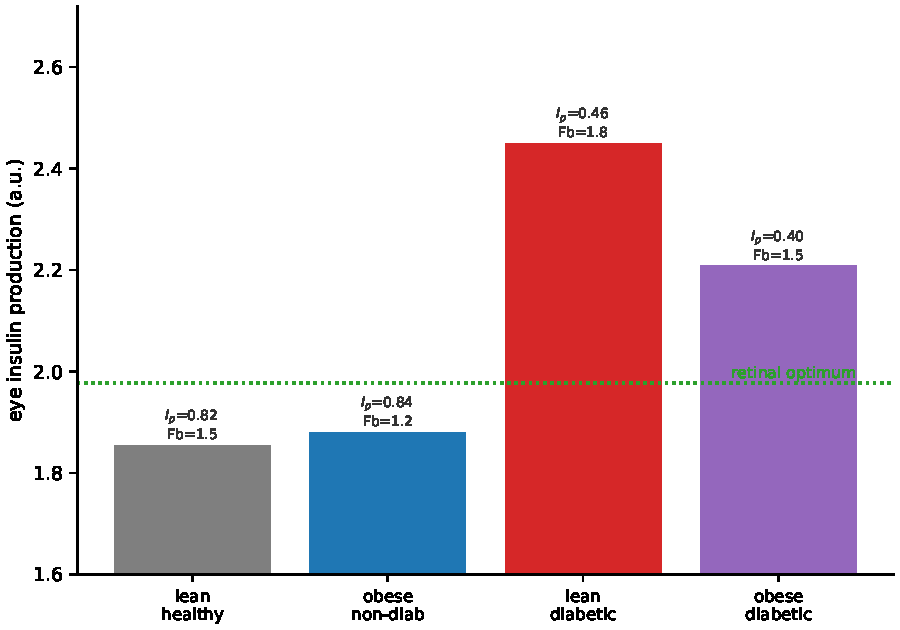
\includegraphics[width=0.72\linewidth]{fig10_eye.pdf}
  \caption{\textbf{Regulated eye insulin near the optimum, decoupled from plasma
  insulin.} Regulated eye insulin across the four clinical conditions (bars), with
  each state's plasma insulin ($I_p$) and blood formate (Fb, mg/L) annotated and
  the retinal optimum marked. Eye insulin \emph{anti}-correlates with plasma
  insulin ($r=-0.90$) and tracks blood one-carbon and local glucose: the
  high-$I_p$ lean-healthy and obese states sit just below the optimum (mild
  deficiency), while the low-$I_p$ lean secretion-defect diabetic --- formate
  overflow plus hyperglycaemia --- is pushed above it into mild excess.}
  \label{fig:eye}
\end{figure}

\subsubsection*{Retinal health: an optimal insulin window}
High formate does something specific in the eye: it drives local insulin toward
its saturated maximum (Fig~\ref{fig:local}). An \emph{excess} of retinal insulin
signalling is itself pathological, on firm evidence. Chronic ocular
over-expression of IGF-1/insulin drives intraocular VEGF and a progression to
proliferative, neovascular retinopathy even without hyperglycaemia~\cite{ruberte2004}; sustained retinal IGF-I causes gliosis, oxidative stress
and neurodegeneration despite being neuroprotective at normal levels~\cite{villacampa2013}; and the ``early worsening'' of retinopathy on intensive
insulin is attributed to insulin acting with VEGF to drive vascular proliferation.
Retinal insulin is thus beneficial in a window and harmful outside it.

We encoded this as a trophic maintenance arm that saturates with local insulin,
minus a pathology arm (VEGF/gliosis/neovascularization) with a higher threshold,
so net retinal health is an inverted-U in local insulin (Fig~\ref{fig:excess}).
Because eye insulin rises with blood formate, retinal health peaks at a
physiological formate ($\sim$5--10~mg/L) and falls off on both sides:
\emph{deficiency} at low formate (obesity's sink, metformin) and \emph{insulin
excess} at high formate (over-supplementation, and the methanol range), where net
health drops to ${\sim}0.24$ against a peak of ${\sim}0.42$. This inverted-U is the
``optimum'' that the homeostat of the previous section targets, and it unifies the
eye story: the retina, like the rest of the body in this model, needs formate ---
and the local insulin it sets --- within an optimal window, with disease at either
end. It notably requires \emph{no} complex-IV inhibition (a mechanism that rests
on sparse, largely in-vitro evidence; see Discussion), resting instead on the
well-supported biology of retinal insulin/IGF excess. It also predicts a mechanism
for diabetic retinopathy orthogonal to hyperglycaemia: a formate/eye-insulin
excess (as in the lean secretion-defect overflow) or deficiency (as in obesity)
could damage the retina at normal plasma insulin.

\begin{figure}[t]
  \centering
  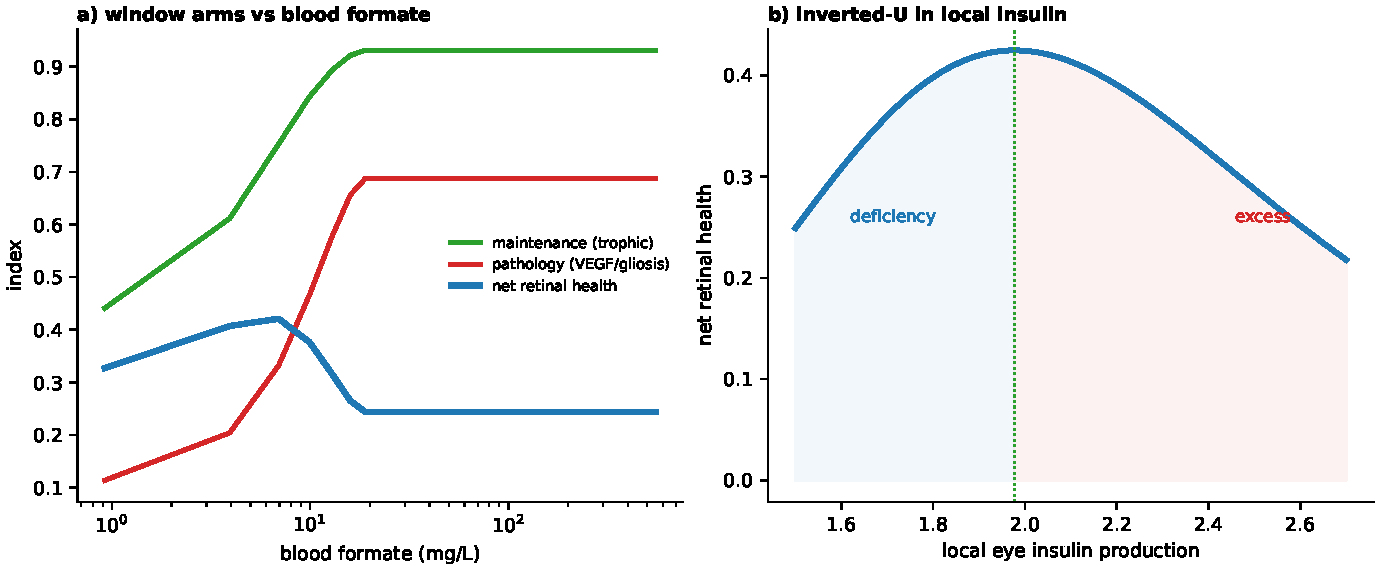
\includegraphics[width=\linewidth]{fig13_insulin_excess.pdf}
  \caption{\textbf{Retinal health is an optimal window in local insulin.} Retinal
  health is scored as a trophic maintenance arm minus a higher-threshold pathology
  arm (VEGF/gliosis/neovascularization); no complex-IV inhibition is invoked. (a) across blood formate, maintenance, pathology and net health (markers at 5, 50, 500~mg/L); (b) net health is an inverted-U in local eye insulin --- both
  deficiency (low formate) and excess (high formate) harm the retina.}
  \label{fig:excess}
\end{figure}

\subsubsection*{Methanol as an acute one-carbon overload}
The same molecule that supports the eye at physiological levels is the toxin of
methanol poisoning at high ones: methanol is oxidised to formate, which
accumulates to the symptomatic ($>50$~mg/L) and lethal ($>500$~mg/L) levels of
intoxication and produces the classic visual loss. In this model that ocular
damage is \emph{insulin excess}, not inhibition of mitochondrial complex~IV: we
leave the respiratory chain uninhibited (the complex-IV route rests on sparse,
largely in-vitro evidence; see Discussion) and let rising formate act only by
driving local insulin past the retinal optimum into the pathological excess zone
(the well-evidenced retinal-health window, Fig~\ref{fig:excess}). We swept blood formate from
physiological to the methanol range for the blood-dependent eye and for the
S6K1-regulated autonomous eye (Fig~\ref{fig:toxlocal}).

Regulation splits the response into two regimes. Across the \emph{physiological}
range the regulated autonomous eye holds insulin at the optimum, so its net
retinal health sits at the peak (${\sim}0.42$) even at low blood formate, whereas
the blood-dependent eye is sub-optimal (deficient) there --- the regulated eye is
protected. But regulation caps the cell's \emph{endogenous} production; it cannot
oppose an \emph{external} formate flood. As blood formate climbs into the methanol
range, circulating formate alone saturates local insulin into excess in both eyes,
and net retinal health collapses to the same insulin-excess floor (${\sim}0.24$).
The two curves are indistinguishable above ${\sim}15$~mg/L. Thus the properly
regulated retina is healthy and buffered under normal one-carbon fluctuations, and
methanol optic toxicity appears as an acute overload that overwhelms that
regulation --- not as a chronic mis-set of local insulin. (As throughout the eye
sections the magnitudes depend on the assumed feedback and window; the robust
content is the two-regime behaviour --- physiological protection, methanol
override.)

\begin{figure}[t]
  \centering
  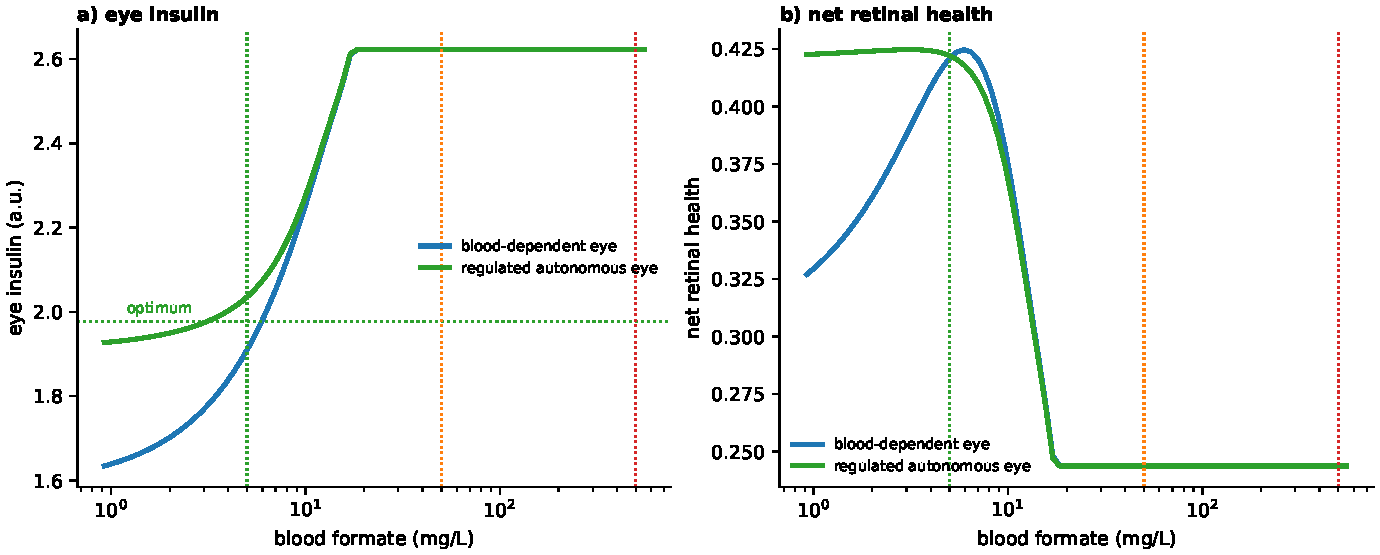
\includegraphics[width=\linewidth]{fig19_methanol_local.pdf}
  \caption{\textbf{Regulated autonomous eye under methanol (insulin-excess only,
  no complex-IV inhibition).} Blood formate swept to the methanol range (log axis;
  markers at 5, 50, 500~mg/L). (a) eye insulin --- the S6K1-regulated autonomous
  eye holds near the optimum at physiological formate, then follows the
  blood-dependent eye up as circulating formate floods in. (b) net retinal health --- the regulated eye is at its healthy peak across the physiological
  range (buffered, unlike the deficient blood-dependent eye) but collapses to the
  same insulin-excess floor once the methanol flood overrides regulation.}
  \label{fig:toxlocal}
\end{figure}

\subsubsection*{Dietary formate and the retina}
With the regulated eye in hand we can place dietary formate on the retinal map.
The formate-limited retinal cell raises its local insulin modestly with dietary
formate (Fig~\ref{fig:dietins}), so the distinctive nutritional prediction of the
formate theory is ocular, not glycaemic, and remains untested. Reassuringly,
dietary eye insulin stays below the retinal optimum --- on the beneficial, rising
limb of the window, well short of the insulin excess that requires the
supra-dietary formate of over-supplementation or methanol. The honest conclusion
is that food formate is real but a minor systemic player, and that ``eat for your
formate'' is, if anything, advice for the retina.

\begin{figure}[t]
  \centering
  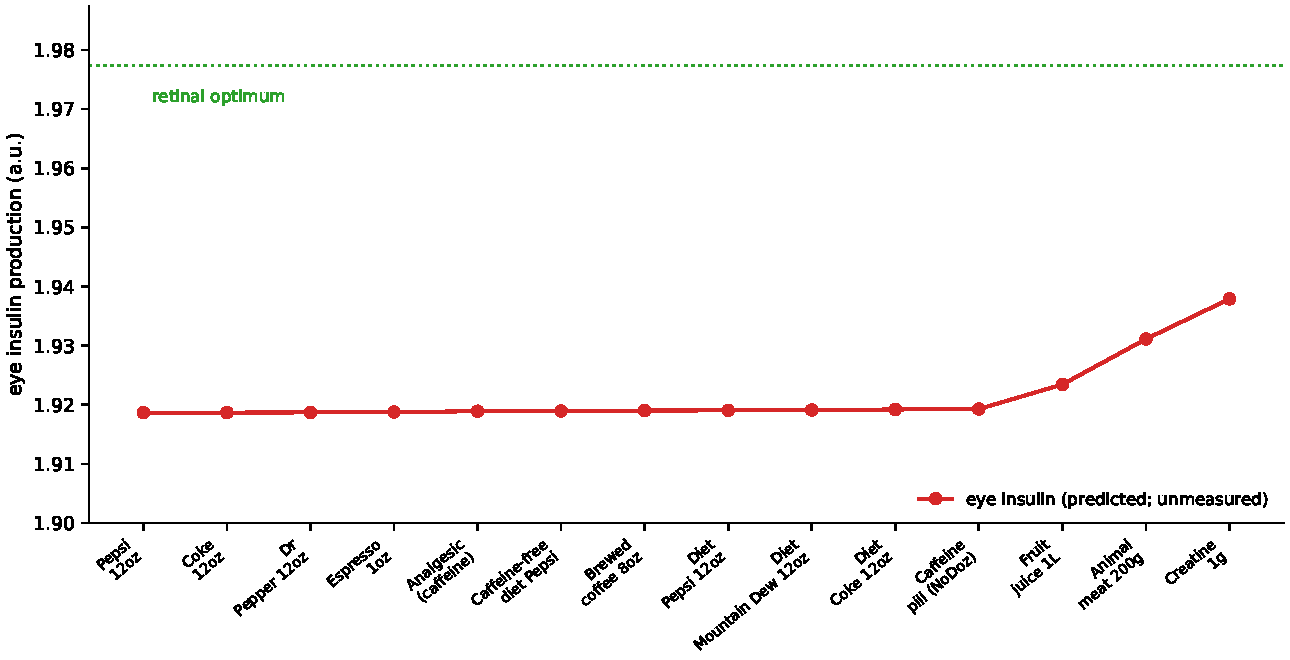
\includegraphics[width=0.68\linewidth]{fig16_eye_insulin.pdf}
  \caption{\textbf{Eye insulin by food (systemic insulin flat).} Predicted eye
  (local retinal) insulin production per food (a.u.); plasma/systemic insulin is
  flat across all foods --- the $\beta$-cell is formate-replete, consistent with
  the measured null effect of creatine and aspartame on fasting insulin --- and is
  not shown. The reference line marks the retinal optimum (peak net retinal
  health). Dietary eye insulin rises modestly with food formate but stays below
  the optimum, on the beneficial limb of the window; it is an untested prediction.}
  \label{fig:dietins}
\end{figure}

\subsection*{Therapeutic implications}
The model's map of formate states points to interventions at each level. We
consider four: two systemic --- nutritional supplementation and metformin --- and
two ocular --- targeting the retina's local formate synthesis, or its insulin
synthesis.

\subsubsection*{Who benefits from formate/serine supplementation?}
Start with the systemic question: would a diabetic patient benefit from formate
(or its precursor serine) supplementation? We swept the dietary intake in
each patient type and read the fasting glucose and the uric-acid side effect
(Fig~\ref{fig:interv}). The answer is conditional on $\beta$-cell formate status.
A \emph{formate-replete} secretion defect does not benefit: the $\beta$-cell is
already formate-saturated, so extra formate does not raise insulin and fasting
glucose is unchanged --- it only raises uric acid. A \emph{formate-deficient}
diabetic $\beta$-cell (low mitochondrial formate: an MTHFD1L variant, antibiotic
or microbiome depletion, or mitochondrial dysfunction) is formate-limited and
\emph{is} rescued: supplementation raised insulin ($+27\,\%$) and lowered fasting
glucose ($7.0\rightarrow6.5$~mM, $-8\,\%$). Obesity blunts this benefit
($-3\,\%$) because the expanded adipose sink competes for the supplemented
formate, and it amplifies the uric-acid side effect ($3.5\rightarrow4.7$ vs
$3.4\rightarrow3.9$~mg/dL in the lean). The model therefore predicts a
\emph{responder phenotype} --- the lean, formate-deficient diabetic --- and a
non-responder / adverse phenotype --- the obese, formate-replete diabetic, in
whom supplementation does not help and worsens hyperuricaemia. It also names the
stratifying measurements: $\beta$-cell/blood formate status (or its causes:
MTHFD1L genotype, recent antibiotics) up front, and serum urate for safety.

\begin{figure}[t]
  \centering
  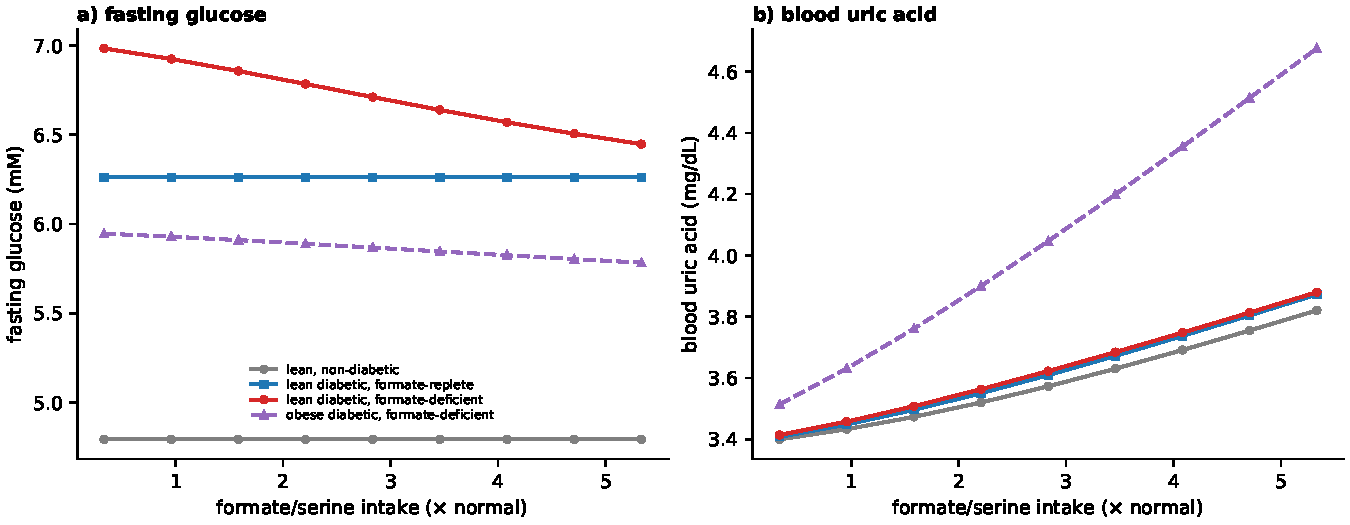
\includegraphics[width=\linewidth]{fig8_intervention.pdf}
  \caption{\textbf{A responder phenotype for formate/serine supplementation.}
  Fasting glucose (a) and blood uric acid (b) versus supplementation dose.
  Only the formate-deficient diabetic $\beta$-cell is rescued (glucose falls);
  the formate-replete diabetic and the non-diabetic do not respond. Obesity blunts
  the glucose benefit (adipose sink competition) and worsens the uric-acid side
  effect.}
  \label{fig:interv}
\end{figure}

\subsubsection*{Metformin: a mitochondrial inhibitor with a dual action}
Metformin --- the antidiabetic drug of the METTEN trial that seeded the
formate--glucose cohort work --- is a mitochondrial complex~I inhibitor and a
PLP-competitive inhibitor of the mitochondrial one-carbon enzyme SHMT2, so it
lowers serine $\rightarrow$ formate flux~\cite{tramonti2021}. We modelled
both actions in the diabetic patient: a peripheral, AMPK-like rise in glucose
effectiveness (its therapeutic arm) and a reduction in mitochondrial formate
production (systemic and $\beta$-cell). Across the dose range (Fig~\ref{fig:metf})
fasting glucose fell ($-8\,\%$ lean, $-5\,\%$ obese) --- yet plasma insulin
\emph{fell} too, and blood formate fell by ${\sim}24\,\%$. The model thus
recovers metformin's defining clinical feature, that it lowers glucose
\emph{without} stimulating insulin (indeed it is insulin-sparing), by locating
the benefit in the peripheral arm; and it predicts, as an experimentally
checkable signature, that metformin \emph{lowers} circulating formate through
SHMT2 inhibition --- opposite in sign to formate supplementation. A corollary
worth flagging is that metformin, by draining mitochondrial formate, could deepen
a pre-existing $\beta$-cell formate deficiency; its net benefit here nonetheless
remains positive because the peripheral arm dominates the fasting glucose.

\begin{figure}[t]
  \centering
  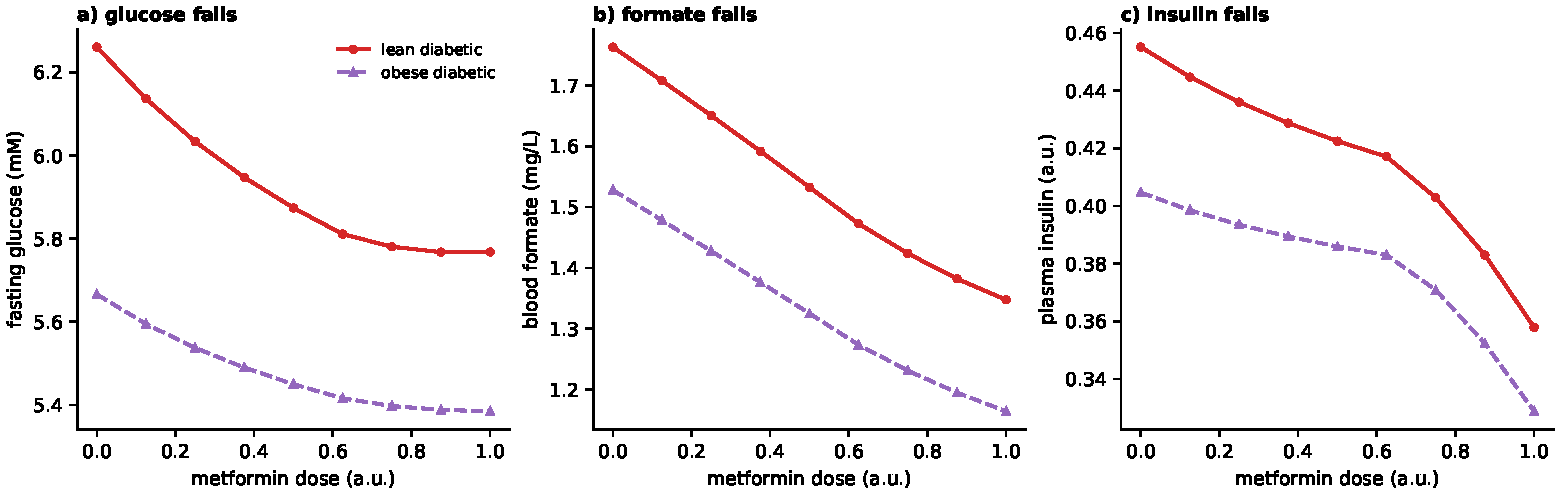
\includegraphics[width=\linewidth]{fig9_metformin.pdf}
  \caption{\textbf{Metformin lowers glucose peripherally while lowering formate
  and insulin.} Dose response in lean and obese diabetics. (a) fasting glucose falls (peripheral/AMPK arm); (b) blood formate falls (SHMT2 inhibition of mitochondrial formate); (c) plasma insulin falls --- metformin is
  insulin-sparing, not a secretagogue.}
  \label{fig:metf}
\end{figure}

\subsubsection*{An intravitreal MTHFD2 inhibitor: a targeted retinal therapy, and a
test of the mechanism}
The regulated eye gives the model a druggable node. MTHFD2, the NAD$^+$-dependent
mitochondrial methylenetetrahydrofolate dehydrogenase/cyclohydrolase, is the entry
enzyme of the pathway that produces the retina's \emph{local} formate (with
MTHFD1L releasing it); it is strongly upregulated in tumours but near-absent in
most normal adult tissue, and potent, selective, orally available inhibitors have
been developed as anticancer agents (e.g.\ DS18561882~\cite{kawai2019}),
with MTHFD2 already flagged as an ocular drug target in retinoblastoma
\cite{yao2025}. In the model an intravitreal MTHFD2 inhibitor scales down
the eye's local mitochondrial formate production (both the endogenous floor and the
ATF4-induced term) while leaving systemic glucose, plasma insulin and
blood-delivered formate untouched --- a local intervention on exactly the
feed-forward of the eye-compartment model. We swept the inhibition from 0 to 100\%
(Fig~\ref{fig:mthfd2}).

The prediction is a precision therapy with a sharp patient-selection rule, and a
clean mechanistic control. In a retina carrying \emph{excess} local insulin --- the
lean secretion-defect overflow with hyperglycaemia, the retinopathy-prone state of
the eye-compartment model (eye insulin ${\sim}2.46$, above the optimum) --- lowering local formate
walks insulin back down through the optimum, and net retinal health rises from
${\sim}0.30$ to its peak ${\sim}0.42$ at ${\sim}70$--$80\%$ inhibition
(Fig~\ref{fig:mthfd2}A,B, red): a local, glucose-sparing route to normalising
insulin-excess retinopathy, distinct from anti-VEGF. But the same drug is
\emph{harmful} to a formate-\emph{deficient} retina (obesity, metformin --- already
below the optimum): it deepens the deficiency, and net health falls from
${\sim}0.42$ to ${\sim}0.19$ (Fig~\ref{fig:mthfd2}B, blue). MTHFD2 inhibition is
thus the mirror image of formate/serine supplementation (above): it helps the
insulin-excess eye and harms the deficient one, and demands the same stratification
by retinal one-carbon/insulin status. Over-inhibition even of an excess retina
eventually overshoots into deficiency, so the effect is dose-limited.

Against methanol optic toxicity the model makes a decisive \emph{negative}
prediction (Fig~\ref{fig:mthfd2}C). Because the toxic formate of methanol
poisoning is generated \emph{systemically} (hepatic oxidation) and floods the
retina across the blood-retinal barrier, it bypasses the retinal MTHFD2 entirely:
at intoxication levels eye insulin and net retinal health are \emph{identical} with
and without the inhibitor (both at the insulin-excess floor ${\sim}0.24$), and at
physiological formate the inhibitor only \emph{worsens} the retina by inducing
local deficiency. An MTHFD2 inhibitor therefore cannot rescue methanol blindness in
this model --- a result that both cleanly separates endogenous (local, druggable)
from exogenous (blood-borne, non-druggable) formate and offers a direct test of the
whole eye mechanism: if retinal insulin excess is the driver, targeting local
formate synthesis should help the diabetic-overflow retina but not the
methanol-flooded one.

\begin{figure}[t]
  \centering
  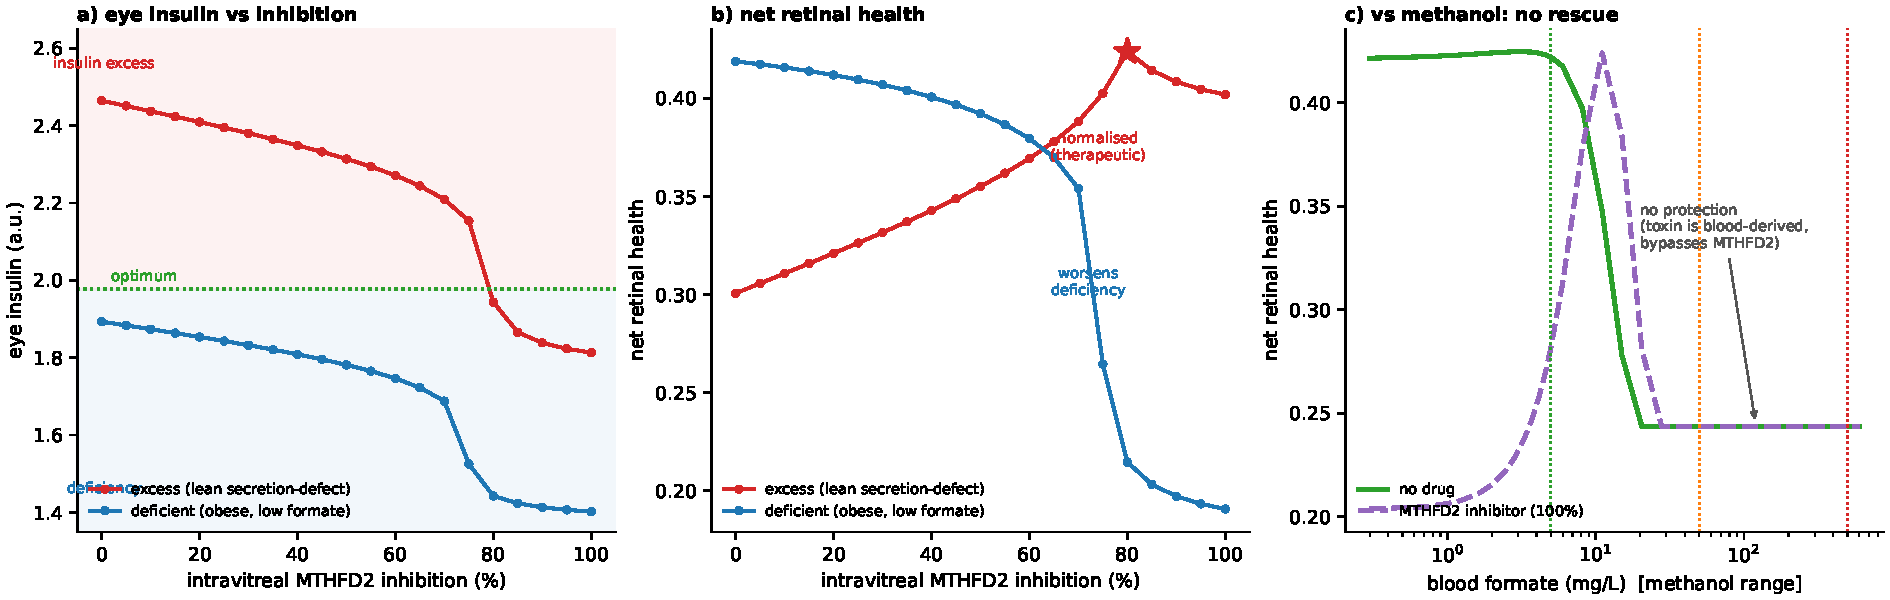
\includegraphics[width=\linewidth]{fig20_mthfd2.pdf}
  \caption{\textbf{An intravitreal MTHFD2 inhibitor normalises insulin-excess
  retinopathy but cannot rescue methanol toxicity.} Retinal MTHFD2 inhibition
  scales down local mitochondrial formate only (blood formate still crosses the
  barrier). (a) Eye insulin falls with inhibition; the excess (lean
  secretion-defect) retina (red) descends through the optimum, the deficient
  (obese/low-formate) retina (blue) into deficiency. (b) Net retinal health:
  partial inhibition (${\sim}70$--$80\%$, star) \emph{normalises} the excess retina
  (therapeutic), while the same dose \emph{worsens} the deficient retina. (c)
  Against a methanol formate flood, the inhibitor gives no protection --- health
  with (dashed) and without (solid) the drug coincide at the insulin-excess floor
  once blood formate overrides local synthesis --- because the toxin is
  blood-derived and bypasses MTHFD2.}
  \label{fig:mthfd2}
\end{figure}

\subsubsection*{An insulin-production inhibitor rescues methanol optic toxicity}
The MTHFD2 inhibitor failed against methanol because it acts \emph{upstream} of the
formate flood; the natural counter-question is whether acting \emph{downstream}, at
the insulin-synthesis node itself, would succeed. In the model insulin production is
mTOR-driven translation, so the direct pharmacology is an mTORC1 inhibitor
(rapamycin/sirolimus), which reduces $\beta$-cell proinsulin biosynthesis
\cite{fraenkel2008} and is available for the eye (intravitreal
sirolimus has been trialled in retinal disease); secretion-blocking classes
(diazoxide on K$_\mathrm{ATP}$, somatostatin analogues such as octreotide, the
latter with intraocular delivery under study) are an alternative acting on release
rather than synthesis. We model the synthesis inhibitor as $\mathrm{mtor\_mult}<1$,
capping the mTOR-driven insulin translation downstream of formate and purine
sensing, and ask how the regulated eye behaves under a methanol load
(Fig~\ref{fig:mtori}).

It rescues the toxicity. Untreated, the eye collapses to the insulin-excess health
floor (${\sim}0.24$) once blood formate exceeds ${\sim}50$~mg/L; a ${\sim}50\%$
intravitreal mTOR inhibitor holds local insulin at the optimum and net retinal
health at its \emph{peak} (${\sim}0.42$) across the entire methanol range, up to
the lethal $500$~mg/L (Fig~\ref{fig:mtori}A, blue). The contrast with the MTHFD2
inhibitor (Fig~\ref{fig:mtori}A, dashed --- indistinguishable from no drug at
intoxication) is the point: because the mTOR inhibitor caps synthesis
\emph{downstream} of the purine/formate signal, it clips a blood-borne overload
that an upstream, formate-directed drug cannot touch. The dose-response at lethal
formate is a therapeutic window (Fig~\ref{fig:mtori}B): health recovers to its
peak at ${\sim}50\%$ inhibition and then declines as over-inhibition overshoots
into deficiency. And the margin is wide: because insulin synthesis has a
mTOR-independent floor and saturates at the top, a proportional mTOR cap
preferentially clips the saturated \emph{excess} while barely moving the
near-optimal physiological eye (net health $0.422\rightarrow0.417$ at physiological
formate; Fig~\ref{fig:mtori}C) --- unlike the MTHFD2 inhibitor, which harmed the
physiological retina. The prediction is therefore specific and testable: during
methanol intoxication an intravitreal insulin-synthesis (mTOR) inhibitor should
preserve retinal function in this insulin-excess model, whereas a local-formate
(MTHFD2) inhibitor should not --- a discriminating experiment for the
insulin-excess mechanism of methanol blindness itself. (As throughout, the
magnitudes depend on the assumed window and feedback; the robust content is the
directionality --- a downstream synthesis block rescues a blood-borne overload that
an upstream block cannot --- and the acute, local nature of the intervention
sidesteps the systemic $\beta$-cell liabilities of chronic mTOR inhibition.)

\begin{figure}[t]
  \centering
  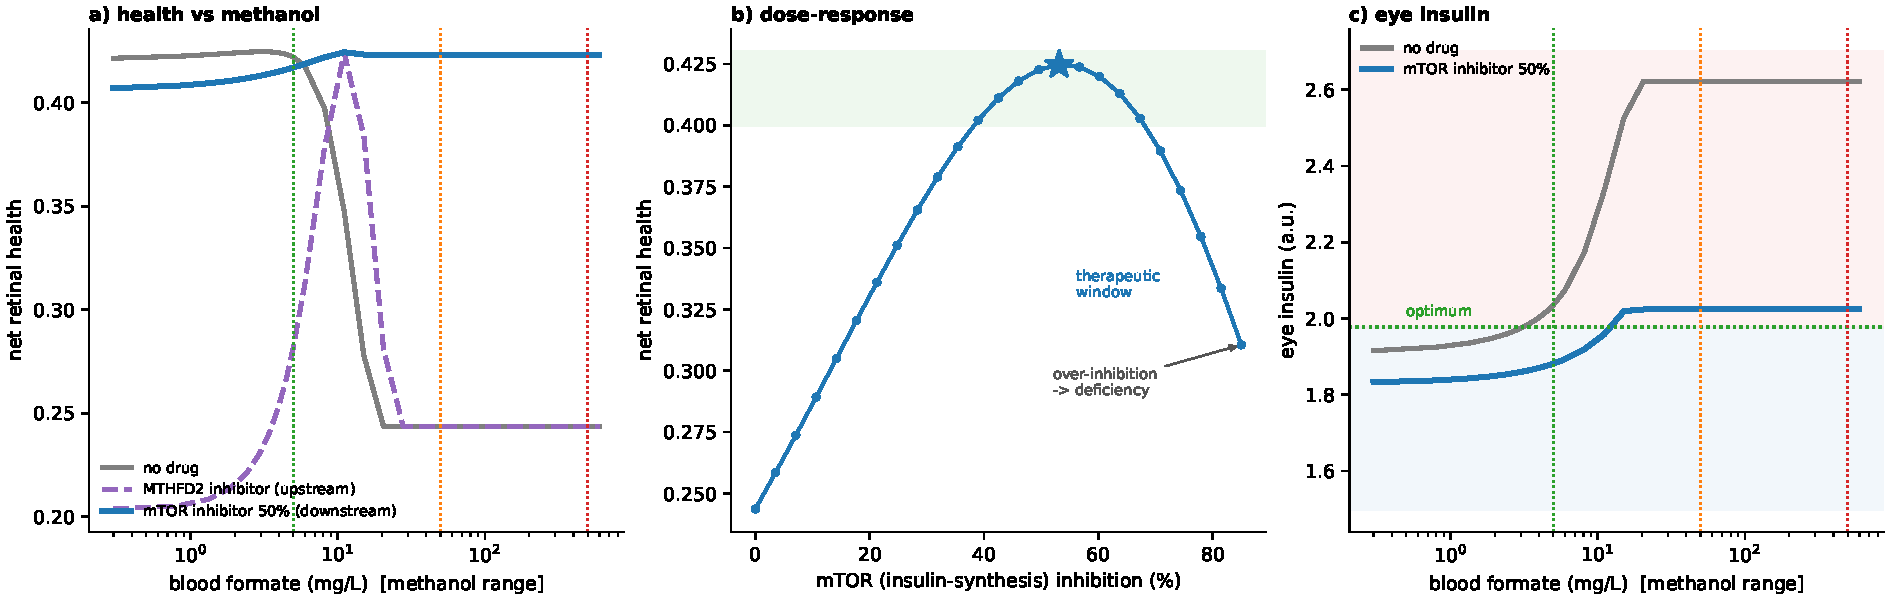
\includegraphics[width=\linewidth]{fig21_mtor_inhibitor.pdf}
  \caption{\textbf{An intravitreal insulin-production (mTOR) inhibitor rescues
  methanol optic toxicity, where the MTHFD2 inhibitor could not.} Insulin synthesis
  is mTOR-driven, so an mTORC1 inhibitor ($\mathrm{mtor\_mult}<1$) caps it
  downstream of the formate flood. (a) Net retinal health vs blood formate: no drug
  (grey) and the upstream MTHFD2 inhibitor (dashed) both collapse to the
  insulin-excess floor at methanol levels, whereas a $50\%$ mTOR inhibitor (blue)
  holds health at the optimum across the whole range. (b) Dose-response at lethal
  methanol ($500$~mg/L): a therapeutic window peaking near $50\%$ inhibition,
  over-inhibition overshooting into deficiency. (c) Eye insulin: the mTOR inhibitor
  clips the methanol excess (down to the optimum) while sparing the near-optimal
  physiological baseline.}
  \label{fig:mtori}
\end{figure}

% ---------------------------------------------------------------------------
\section*{Discussion}
A kinetic model shows that the proposed formate $\rightarrow$ purine
$\rightarrow$ mTOR $\rightarrow$ insulin chain is quantitatively coherent and,
once the glucose--insulin axis is calibrated to islet data, yields non-trivial
predictions: a formate dose-response of insulin synthesis, a ${\sim}45\,\%$
insulin deficit under mitochondrial formate loss, coupled uric-acid changes, and
dietary rescue. The sensitivity analysis pinpoints the mTOR purine-sensing Hill
coefficient and the mitochondrial formate capacity as the parameters most in
need of measurement.

Absolute insulin quantities are now anchored: scaling the granule pool to the
measured $\beta$-cell insulin content (${\sim}20$~pg/cell) gives a stimulated
secretion of ${\sim}16$~pg/cell/h (${\sim}2.8$~fmol/cell/h), of the expected
order; this single scale does not affect any calibrated ratio. The peripheral
alternative, previously untested, is now represented explicitly in the
whole-body loop and yields the plasma-insulin discriminator above. Two caveats
remain. First, the insulin-secretion and purine-degradation kinetics outside the
reused core are still scaled rather than individually fitted, though the
sensitivity analysis shows the predictions do not depend on them. Second, the
whole-body layer is a minimal (Bergman-type) representation; a physiological
multi-tissue model would refine the quantitative split. The discriminating
experiment stands regardless: measure plasma insulin (and, in islets,
proinsulin/\textit{INS} translation across a formate gradient, and GSIS in
MTHFD1L-deficient islets) during formate supplementation.

\emph{Confrontation with existing data.} A survey of candidate test datasets finds the mTOR $\rightarrow$ insulin arm
strongly supported (Raptor/\allowbreak TSC2 $\beta$-cell models; rapamycin)~\cite{ni2017,blandino2017,fraenkel2008} and folate/\allowbreak
one-carbon deficiency impairing $\beta$-cell insulin biosynthesis~\cite{hsu2013},
but also two findings in tension with the model that must be addressed. First, in
islets, acute knockdown of the mitochondrial one-carbon pathway (SHMT2/\allowbreak MTHFD2)
\emph{increases} glucose-stimulated secretion while its ATF4-driven induction
raises insulin \emph{content} but lowers secretion~\cite{pelligra2023} --- a
synthesis-versus-secretion dissociation that this model is built to represent and
that argues for measuring content/translation, not only GSIS. Second, a large
prospective cohort reports \emph{higher} circulating formate with incident
diabetes (opposite the ``low-formate'' reading of Pietzke et al.~\cite{pietzke2019}); as shown above
(Fig~\ref{fig:diab}) the model reproduces this through the secretion-defect
overflow route, and the cohort's own data (formate independent of genetic risk
and not a risk mediator) place formate as a consequence marker, consistent with
that route. Higher serum urate likewise associates with diabetes although
Mendelian randomization is null --- so the urate arm is best read as a flux marker
of purine turnover, not a health claim. Each remains an open test that the paired
measurements above would settle.

% ---------------------------------------------------------------------------
\section*{Materials and methods}
This section summarises the models; S1 Appendix gives the complete
specification --- every state variable, rate law, ODE balance, parameter value with
provenance, calibration procedure and the monostability analysis (Fig A in S1 Appendix).
Fifteen ODEs (ATP, ADP, AMP, formate, 10-CHO-THF, PRPP, GAR, AICAR, IMP,
adenylosuccinate, guanine nucleotides, hypoxanthine/xanthine, urate, pro-insulin,
insulin) with
mass-action/MM/Hill rate laws; time unit hours, concentrations mM (insulin in
arbitrary units). Integrated with an implicit solver (BDF); steady states from a
pre-integration followed by a log-space least-squares polish (residuals
$<10^{-13}$~mM/h). The purine/energy core and the PPAT--NUDT5 glue calibration
are inherited from Formate-NUDT5~\cite{vazqueznudt5}; GSIS parameters were
fitted here by least squares to EC$_{50}$ and stimulation-index targets.
Insulin quantities are converted to per-cell units by one scale anchoring the
granule pool to the measured $\beta$-cell insulin content. The whole-body loop
(\texttt{WholeBody}) embeds the $\beta$-cell as the insulin source of a
Bergman minimal model (glucose effectiveness $S_g$, insulin sensitivity $S_i$,
remote insulin action), with per-hour rate constants; the peripheral formate
effect is a fractional increase in $S_g$. For the diabetes-paradox analysis
(\texttt{FormateDiabetes}) blood formate is an additional dynamic pool fed by
dietary intake and endogenous production and drained by an insulin-scaled
consumption term and renal clearance, and the secretion defect scales plasma
insulin appearance. The obesity analysis (\texttt{CoupledModel}) adds a
third compartment --- an adipocyte metabolic model (\texttt{AdipocyteModel}, ten
ODEs: the shared energy and one-carbon/purine modules with insulin-dependent
glucose uptake and lipid storage, and XOR-mediated urate secretion) --- coupled
to the $\beta$-cell through shared blood glucose, insulin, formate and urate
pools; obesity scales adipose mass, XOR and insulin resistance, and the supplementation
analysis sweeps the dietary intake with the $\beta$-cell held formate-replete or
formate-deficient. Metformin is modelled as a rise in glucose effectiveness
(peripheral/AMPK) together with a reduction in mitochondrial formate production
(systemic and $\beta$-cell), representing SHMT2 inhibition. The eye compartment
(\texttt{EyeModel}) is a retinal insulin cell using the $\beta$-cell machinery
driven by blood glucose and formate with a low endogenous mitochondrial formate
and strictly local insulin (no plasma exchange). Local formate production is an
ATF4-style feed-forward on the cell's own mTOR/insulin signal, capped by an
mTORC1--S6K1--IRS-1 negative feedback; feed-forward steady states are obtained by
integrating to the stable attractor (not root-polished, which can return
dynamically unstable fixed points), and the regulated eye was verified monostable
by basin tests and a self-consistency/bifurcation analysis
(\texttt{eye\_bifurcation.py}). Retinal health is a trophic-maintenance minus
higher-threshold pathology (VEGF/gliosis) inverted-U in local insulin; methanol is
modelled purely as this insulin-excess overload, with no complex-IV inhibition.
Parameters carry provenance tags [PUB]/[FIT]/[LIT]/[ASM]. The eye analyses (local
retinal insulin, the insulin-excess optimal window, methanol overload, and the
regulated local formate feed-forward) use \texttt{EyeModel}; the dietary
meta-analysis maps the
per-food formate content to model intake and compares model predictions with
pooled literature estimates. The model is implemented as an object-oriented class
hierarchy in \texttt{model.py}: a \texttt{MetabolicCell} base (shared BDF
integration, log-space steady state, and rate-law primitives) subclassed by
\texttt{BetaCellModel}, \texttt{AdipocyteModel} and \texttt{EyeModel}, with
\texttt{WholeBody}, \texttt{FormateDiabetes}, \texttt{CoupledModel} and its gut-microbiome extension \texttt{GutUrateCycle} containers;
each compartment carries an explicit parameter dataclass. Code, calibrated outputs
(\texttt{data/*.csv}) and figure generators (\texttt{make\_figs.py},
\texttt{make\_body.py}, \texttt{make\_diet.py}, \texttt{make\_eye\_figs.py},
\texttt{make\_mthfd2.py}, \texttt{make\_mtor\_inhibitor.py},
\texttt{eye\_bifurcation.py}, \texttt{make\_supp\_bif.py}) are in this repository.

\begin{table}[h]
  \centering
  \small
  \caption{Key numbers (this run).}
  \begin{tabular}{@{}lr@{}}
    \toprule
    Quantity & Value \\
    \midrule
    ATP/ADP, 1$\rightarrow$10 mM glucose~\cite{detimary1998} & 2.4$\rightarrow$11.6 (target 2.4/11.6) \\
    IMP / S-AMP, low $\rightarrow$ high glucose~\cite{gooding2015} & $\times$0.28 / $\times$3.4 (target 0.23/3.4) \\
    Raptor-KO insulin content~\cite{ni2017} & 50\% of WT (target 50\%) \\
    GSIS EC$_{50}$ / stimulation index & 8.0 mM / 5.5 (targets 8.0 / 5.5) \\
    Insulin synthesis, formate $0\rightarrow2$ mM (11 mM glucose) & $+66\,\%$ \\
    Insulin synthesis loss, mito-formate $100\%\rightarrow0\%$ & ${\sim}45\,\%$ \\
    mTOR, mito-formate $100\%\rightarrow0\%$ & $0.35\rightarrow0.03$ \\
    Urate secretion, mito-formate $100\%\rightarrow0\%$ & $0.10\rightarrow0.02$ mM/h \\
    Insulin content / secretion (absolute) & 20 pg/cell / 16 pg/cell/h \\
    Central formate: $\Delta$glucose AUC / $\Delta$insulin AUC & $-21\,\%$ / $+20\,\%$ \\
    Peripheral formate: $\Delta$glucose AUC / $\Delta$insulin AUC & $-14\,\%$ / $-2\,\%$ \\
    Blood formate: obesity / diabetes (vs healthy) & $-14\,\%$ / $+21\,\%$ \\
    Supplementation: $\Delta$glucose, deficient / replete diabetic & $-8\,\%$ / $0\,\%$ \\
    Metformin: $\Delta$glucose / $\Delta$blood formate & $-8\,\%$ / $-24\,\%$ \\
    Eye insulin: corr.\ with blood formate / plasma insulin & $+0.89$ / $-0.90$ \\
    Regulated eye: retinal health, physiological / methanol range & $0.42$ (peak) / $0.24$ (floor) \\
    Diet: corr(food formate, T2D log-RR) & $-0.02$ (no relationship) \\
    \bottomrule
  \end{tabular}
\end{table}
\section*{Supporting information}

\paragraph*{S1 Appendix.}
\label{S1_Appendix}
\textbf{Supplementary methods and full model specification.} Complete
specification of every state variable, rate law, ODE balance and parameter value
with provenance; the calibration procedure; and the monostability analysis of the
regulated eye (basin tests and self-consistency/bifurcation analysis, Fig A).

\section*{Acknowledgments}
Nodes \& Links Ltd provided support in the form of salary for Alexei Vazquez, but
did not have any additional role in the conceptualization of the study, analysis,
decision to publish, or preparation of the manuscript. The code and text were
prepared with the assistance of Claude Opus~4.8, an AI assistant developed by
Anthropic.

\section*{Data availability}
All code, calibrated data outputs and figure-generating scripts underlying the
results are openly available in the accompanying project repository: the
object-oriented model (\texttt{model.py}), the figure generators
(\texttt{make\_*.py}, \texttt{eye\_bifurcation.py}) and the calibrated outputs
(\texttt{data/*.csv}). Repository: \url{https://github.com/av2atgh/formate}
(archived at Zenodo, DOI to be assigned on submission).

\section*{Competing interests}
AV is a paid employee of Nodes \& Links Ltd. This does not alter the author's
adherence to PLOS Computational Biology policies on sharing data and materials.

\nolinenumbers

\bibliography{formate_insulin}

\end{document}
